\documentclass[12pt,a4paper]{article}

% --- Page Layout -------------------------------------------------------------
\usepackage[a4paper, margin=0.8in, headheight=14pt]{geometry}

% --- Fonts (XeLaTeX) ---------------------------------------------------------
\usepackage{fontspec}
\usepackage{unicode-math}
\setmainfont{TeX Gyre Pagella}
\setmonofont[Scale=0.88]{TeX Gyre Cursor}
\setmathfont{Latin Modern Math}

% --- Packages ---------------------------------------------------------------
\usepackage{xcolor}
\usepackage{titlesec}
\usepackage{enumitem}
\usepackage{tabularx}
\usepackage{booktabs}
\usepackage{array}
\usepackage{amsmath}
\usepackage{tikz}
\usetikzlibrary{shapes.geometric, arrows.meta, positioning, calc, fit, decorations.pathreplacing, decorations.pathmorphing}
\usepackage{tcolorbox}
\tcbuselibrary{skins, breakable}
\usepackage{hyperref}
\usepackage{fancyhdr}
\usepackage{graphicx}
\usepackage{microtype}
\hyphenpenalty=10000
\exhyphenpenalty=10000
\sloppy
\usepackage{caption}
\usepackage{setspace}
\usepackage{multirow}
\usepackage{tocloft}

% --- Q&A helper --------------------------------------------------------------
\newcommand{\Q}[1]{\textbf{#1}\par\noindent\ignorespaces}

% --- Colour Palette ----------------------------------------------------------
\definecolor{myred}{RGB}{196,30,58}
\definecolor{mydark}{RGB}{30,30,50}
\definecolor{mygreen}{RGB}{14,120,80}
\definecolor{myteal}{RGB}{0,130,140}
\definecolor{myamber}{RGB}{180,100,0}
\definecolor{mypurple}{RGB}{100,30,160}
\definecolor{mygray}{RGB}{246,247,249}
\definecolor{mgframe}{RGB}{180,185,200}
\definecolor{watermark}{RGB}{145,150,170}
\definecolor{hdrred}{RGB}{250,232,235}
\definecolor{hdrgreen}{RGB}{220,244,233}
\definecolor{hdrteal}{RGB}{220,242,244}
\definecolor{hdramber}{RGB}{253,242,215}
\definecolor{hdrpurple}{RGB}{238,228,255}
\definecolor{hdrgray}{RGB}{238,240,245}
\definecolor{rowalt}{RGB}{250,251,253}

% --- Section Formatting ------------------------------------------------------
\titleformat{\section}
  {\large\bfseries\color{myred}}{\thesection.}{0.5em}{}
  [\vspace{1pt}{\color{myred}\rule{\linewidth}{0.8pt}}]
\titleformat{\subsection}
  {\normalsize\bfseries\color{myteal}}{\thesubsection}{0.5em}{}
\titlespacing*{\section}{0pt}{18pt}{7pt}
\titlespacing*{\subsection}{0pt}{11pt}{4pt}

% --- Paragraph ---------------------------------------------------------------
\setlength{\parindent}{0pt}
\setlength{\parskip}{4pt}

% --- Page filling ------------------------------------------------------------
% Use \raggedbottom so long breakable tcolorboxes don't leave nearly blank
% pages when they refuse to split. Pages end at natural content height.
\raggedbottom

% --- TOC Styling -------------------------------------------------------------
\renewcommand{\cfttoctitlefont}{\large\bfseries\color{myred}}
\renewcommand{\cftaftertoctitle}{\par\noindent{\color{myred}\rule{\linewidth}{0.8pt}}}
\setlength{\cftbeforetoctitleskip}{0pt}
\setlength{\cftaftertoctitleskip}{6pt}
\renewcommand{\cftsecfont}{\normalsize\bfseries\color{mydark}}
\renewcommand{\cftsecpagefont}{\normalsize\bfseries\color{mydark}}
\renewcommand{\cftsecleader}{\cftdotfill{\cftdotsep}}
\setlength{\cftbeforesecskip}{7pt}
\renewcommand{\cftsubsecfont}{\small\color{mydark}}
\renewcommand{\cftsubsecpagefont}{\small\color{mydark}}
\setlength{\cftbeforesubsecskip}{3pt}
\setlength{\cftsubsecindent}{1.4em}

% --- Table helpers -----------------------------------------------------------
\renewcommand{\arraystretch}{1.45}
\setlength{\tabcolsep}{6pt}
\newcolumntype{B}[1]{>{\small\bfseries\raggedright\arraybackslash}m{#1}}
\newcolumntype{Y}{>{\small\raggedright\arraybackslash}X}
\renewcommand{\tabularxcolumn}[1]{m{#1}}

% --- Header / Footer ---------------------------------------------------------
\pagestyle{fancy}
\fancyhf{}
\fancyhead[L]{\small\color{myred}\textbf{BS-CH101}\;\color{mydark}--- Chemistry-I}
\fancyhead[R]{\small\color{myteal}\textbf{Module 2 Notes}}
\fancyfoot[C]{\small\color{mydark}\thepage}
\fancyfoot[R]{\small\color{watermark}\textit{\copyright\ Biraj}}
\renewcommand{\headrulewidth}{0.5pt}
\renewcommand{\footrulewidth}{0.3pt}

% --- Hyperref ---------------------------------------------------------------
\hypersetup{
  colorlinks=true, linkcolor=myteal, urlcolor=myteal,
  pdfauthor={Biraj Sarkar},
  pdftitle={BS-CH101 --- Module 2 Notes: Spectroscopic Techniques and Applications}
}

% --- tcolorbox styles --------------------------------------------------------
\tcbset{
  tikzbox/.style={
    colback=mygray, colframe=mgframe, boxrule=0.6pt, arc=4pt,
    left=8pt, right=8pt, top=6pt, bottom=6pt,
    colbacktitle=mgframe, coltitle=mydark,
    fonttitle=\small\bfseries
  },
  defbox/.style={
    colback=hdrgreen, colframe=mygreen, boxrule=0.8pt, arc=4pt,
    left=9pt, right=9pt, top=6pt, bottom=6pt,
    colbacktitle=mygreen, coltitle=white,
    fonttitle=\small\bfseries
  },
  formulabox/.style={
    colback=hdrteal, colframe=myteal, boxrule=0.8pt, arc=4pt,
    left=9pt, right=9pt, top=7pt, bottom=7pt,
    colbacktitle=myteal, coltitle=white,
    fonttitle=\small\bfseries
  },
  examplebox/.style={
    colback=hdramber, colframe=myamber, boxrule=0.8pt, arc=4pt,
    left=9pt, right=9pt, top=6pt, bottom=6pt,
    colbacktitle=myamber, coltitle=white,
    fonttitle=\small\bfseries
  },
  masonbox/.style={
    colback=hdrpurple, colframe=mypurple, boxrule=0.8pt, arc=4pt,
    left=9pt, right=9pt, top=6pt, bottom=6pt,
    colbacktitle=mypurple, coltitle=white,
    fonttitle=\small\bfseries
  },
  exambox/.style={
    colback=hdrpurple, colframe=mypurple, boxrule=1pt, arc=5pt,
    left=10pt, right=10pt, top=8pt, bottom=8pt,
    colbacktitle=mypurple, coltitle=white,
    fonttitle=\bfseries,
    breakable, title after break={\textbf{Frequently Asked / Viva Questions (contd.)}}}
}
\tcbset{breakable}

% --- TikZ styles -------------------------------------------------------------
\tikzset{
  block/.style={rectangle, draw=myteal, fill=hdrteal,
    text width=2.4cm, align=center, minimum height=0.95cm,
    font=\small, rounded corners=3pt, line width=0.7pt},
  redblock/.style={rectangle, draw=myred, fill=hdrred,
    text width=2.4cm, align=center, minimum height=0.95cm,
    font=\small, rounded corners=3pt, line width=0.7pt},
  netnode/.style={rectangle, draw=myteal, fill=hdrteal,
    text width=1.5cm, align=center, minimum height=0.8cm,
    font=\small, rounded corners=3pt, line width=0.7pt},
  sumjunc/.style={circle, draw=myamber, fill=hdramber,
    minimum size=0.62cm, font=\small, line width=0.8pt},
  snode/.style={circle, draw=mypurple, fill=hdrpurple,
    minimum size=0.55cm, font=\footnotesize, line width=0.7pt},
  arrow/.style={-Stealth, thick, color=mydark},
  redarrow/.style={-Stealth, thick, color=myred},
  line/.style={thick, color=mydark}
}

\begin{document}

\begin{center}
  {\LARGE\bfseries\color{myred} BS-CH101 / BS-CH201 --- Chemistry-I}\\[5pt]
  {\normalsize\color{mydark} Semester I/II \quad$\bullet$\quad 3L:1T:0P \quad$\bullet$\quad 4 Credits}\\[3pt]
  {\normalsize\color{myteal}\textbf{Module 2 Exam Notes: Spectroscopic Techniques and Applications}}\\[3pt]
  {\small\color{mydark} CGEC \;$|$\; B.Tech ECE (2023--27) \;$|$\; \textit{Biraj Sarkar}}
\end{center}
\vspace{2pt}
\noindent{\color{myred}\rule{\linewidth}{1.5pt}}
\vspace{2pt}

\hypersetup{linkcolor=mydark}
\tableofcontents
\hypersetup{linkcolor=myteal}
\newpage
% ===============================================================================
\section{Principles of Spectroscopy and Selection Rules}
% ===============================================================================

\begin{tcolorbox}[defbox]
\textbf{Spectroscopy} is the branch of science that studies the interaction of electromagnetic radiation with matter. The pattern of absorbed, emitted, or scattered radiation gives a fingerprint of the molecular structure, energy levels, and dynamics of the sample.
\end{tcolorbox}

\subsection{Electromagnetic Radiation and Its Quantum Nature}
Electromagnetic (EM) radiation behaves both as a wave and as a stream of photons. As a wave, it is described by frequency $\nu$, wavelength $\lambda$, and wavenumber $\bar{\nu}$. As a particle, each photon carries a discrete amount of energy $E=h\nu$.

\begin{tcolorbox}[formulabox, title={Wave--Particle Relations}]
\[
c = \nu\lambda, \qquad \bar{\nu}=\frac{1}{\lambda}=\frac{\nu}{c}, \qquad E=h\nu=\frac{hc}{\lambda}=hc\bar{\nu}
\]
\textbf{Symbols:} $c=3\times10^{8}\ \mathrm{m\,s^{-1}}$ (speed of light); $h=6.626\times10^{-34}\ \mathrm{J\,s}$ (Planck constant); $\lambda$ in m; $\nu$ in Hz; $\bar{\nu}$ in $\mathrm{cm^{-1}}$ when $\lambda$ is in cm.
\end{tcolorbox}

\subsection{The Electromagnetic Spectrum and Spectroscopic Regions}
Different regions of the EM spectrum probe different molecular motions because each region carries an energy that matches a specific kind of energy gap.

\begin{tcolorbox}[tikzbox, title={Electromagnetic Spectrum: Energy Increases Left to Right}]
\centering
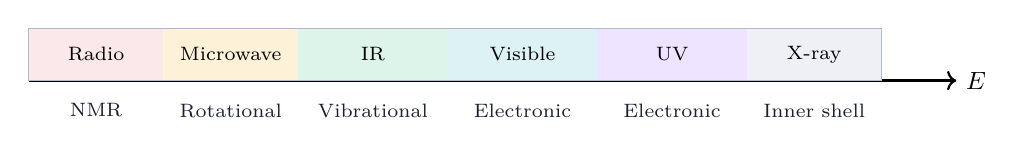
\begin{tikzpicture}[scale=0.95]
  % Energy axis
  \draw[->, thick] (0,0) -- (12.4,0) node[right, font=\small] {$E$};
  % Region bands
  \fill[hdrred]    (0.0,0) rectangle (1.8,0.7);
  \fill[hdramber]  (1.8,0) rectangle (3.6,0.7);
  \fill[hdrgreen]  (3.6,0) rectangle (5.6,0.7);
  \fill[hdrteal]   (5.6,0) rectangle (7.6,0.7);
  \fill[hdrpurple] (7.6,0) rectangle (9.6,0.7);
  \fill[hdrgray]   (9.6,0) rectangle (11.4,0.7);
  \draw[mgframe] (0,0) rectangle (11.4,0.7);
  % Region labels
  \node[font=\scriptsize] at (0.9,0.35)  {Radio};
  \node[font=\scriptsize] at (2.7,0.35)  {Microwave};
  \node[font=\scriptsize] at (4.6,0.35)  {IR};
  \node[font=\scriptsize] at (6.6,0.35)  {Visible};
  \node[font=\scriptsize] at (8.6,0.35)  {UV};
  \node[font=\scriptsize] at (10.5,0.35) {X-ray};
  % Transition labels under
  \node[font=\scriptsize, color=mydark] at (0.9,-0.40)  {NMR};
  \node[font=\scriptsize, color=mydark] at (2.7,-0.40)  {Rotational};
  \node[font=\scriptsize, color=mydark] at (4.6,-0.40)  {Vibrational};
  \node[font=\scriptsize, color=mydark] at (6.6,-0.40)  {Electronic};
  \node[font=\scriptsize, color=mydark] at (8.6,-0.40)  {Electronic};
  \node[font=\scriptsize, color=mydark] at (10.5,-0.40) {Inner shell};
\end{tikzpicture}
\end{tcolorbox}

\textbf{Region--energy mapping:}\par\noindent
\begin{tabularx}{\linewidth}{|B{2.6cm}|Y|Y|Y|}
\hline
\textbf{Region} & \textbf{Wavelength} & \textbf{Energy / quantum} & \textbf{Type of transition} \\
\hline
Radio  & $1\ \mathrm{m}$--$10\ \mathrm{km}$ & very low ($\mu\mathrm{eV}$) & Nuclear spin flip (NMR) \\
\hline
Microwave & $1\ \mathrm{mm}$--$1\ \mathrm{m}$ & $10^{-5}$--$10^{-3}\ \mathrm{eV}$ & Rotational (also ESR) \\
\hline
Infrared (IR) & $700\ \mathrm{nm}$--$1\ \mathrm{mm}$ & $10^{-3}$--$1\ \mathrm{eV}$ & Vibrational \\
\hline
Visible & $400$--$700\ \mathrm{nm}$ & $1.7$--$3.1\ \mathrm{eV}$ & Outer electronic \\
\hline
Ultraviolet (UV) & $10$--$400\ \mathrm{nm}$ & $3.1$--$124\ \mathrm{eV}$ & Outer electronic \\
\hline
X-ray & $0.01$--$10\ \mathrm{nm}$ & $0.1$--$100\ \mathrm{keV}$ & Inner-shell, diffraction \\
\hline
$\gamma$-ray & $<0.01\ \mathrm{nm}$ & $>100\ \mathrm{keV}$ & Nuclear (Mossbauer) \\
\hline
\end{tabularx}

\subsection{Absorption, Emission and Scattering}
Three primary photon-matter events form the basis of every spectroscopic experiment.

\begin{tcolorbox}[tikzbox, title={Three Photon--Matter Processes}]
\centering
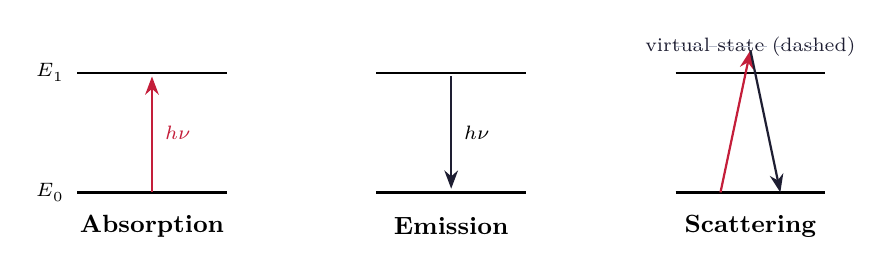
\begin{tikzpicture}[scale=0.95]
  % Absorption
  \draw[thick] (0,0) -- (2.0,0); \node[font=\scriptsize, anchor=east] at (-0.05,0) {$E_0$};
  \draw[thick] (0,1.6) -- (2.0,1.6); \node[font=\scriptsize, anchor=east] at (-0.05,1.6) {$E_1$};
  \draw[redarrow] (1.0,0) -- (1.0,1.55);
  \node[font=\scriptsize, color=myred, anchor=west] at (1.05,0.8) {$h\nu$};
  \node[font=\small\bfseries] at (1.0,-0.45) {Absorption};

  % Emission
  \draw[thick] (4.0,0) -- (6.0,0);
  \draw[thick] (4.0,1.6) -- (6.0,1.6);
  \draw[arrow] (5.0,1.55) -- (5.0,0.05);
  \node[font=\scriptsize, anchor=west] at (5.05,0.8) {$h\nu$};
  \node[font=\small\bfseries] at (5.0,-0.45) {Emission};

  % Scattering
  \draw[thick] (8.0,0) -- (10.0,0);
  \draw[thick] (8.0,1.6) -- (10.0,1.6);
  \node[font=\scriptsize, color=mydark] at (9.0,1.95) {virtual state (dashed)};
  \draw[dashed, mgframe] (8.0,1.95) -- (10.0,1.95);
  \draw[redarrow] (8.6,0) -- (9.0,1.9);
  \draw[arrow] (9.0,1.9) -- (9.4,0);
  \node[font=\small\bfseries] at (9.0,-0.45) {Scattering};
\end{tikzpicture}
\end{tcolorbox}

\textbf{Quick comparison:}\par\noindent
\begin{tabularx}{\linewidth}{|B{2.6cm}|Y|Y|Y|}
\hline
\textbf{Process} & \textbf{What happens} & \textbf{Detected as} & \textbf{Examples} \\
\hline
Absorption & Photon raises molecule from low to high state & Loss of intensity at $\nu$ & UV-Vis, IR \\
\hline
Emission & Excited molecule drops back, releasing photon & Light at characteristic $\nu$ & Fluorescence, AES \\
\hline
Scattering & Photon redirected (with or without energy change) & Light at angle from beam & Raman, X-ray scattering \\
\hline
\end{tabularx}

\subsection{Resonance Condition and the Bohr Frequency Rule}
A photon is absorbed only when its energy matches the gap between two molecular energy levels. This is the \emph{resonance condition}.

\begin{tcolorbox}[formulabox, title={Bohr Frequency Condition}]
\[
\Delta E = E_2 - E_1 = h\nu = \frac{hc}{\lambda} = hc\bar{\nu}
\]
Only photons with this exact $\nu$ are absorbed. Off-resonance photons pass through unchanged. This is why spectra show \emph{discrete lines or bands} instead of a continuum.
\end{tcolorbox}

\subsection{Selection Rules: Allowed and Forbidden Transitions}
Even when the resonance condition is satisfied, a transition occurs only if the corresponding selection rule is obeyed. Selection rules come from the requirement that the transition dipole moment integral be non-zero.

\begin{tcolorbox}[formulabox, title={Transition Probability and Dipole Moment}]
\[
P_{1\to2} \propto |\,\mu_{12}\,|^{2}, \qquad
\mu_{12}=\int \psi_2^{*}\,\hat{\mu}\,\psi_1\,d\tau
\]
\textbf{Allowed} transition: $\mu_{12}\neq 0$ — strong band, high intensity.\\
\textbf{Forbidden} transition: $\mu_{12}=0$ in the simple model — band absent or very weak.
\end{tcolorbox}

\textbf{Two general selection rules:}
\begin{enumerate}[leftmargin=*, itemsep=2pt, topsep=2pt]
  \item \textbf{Gross selection rule:} The molecule must possess a property (e.g.\ permanent or oscillating dipole) capable of interacting with the radiation.
  \item \textbf{Specific selection rule:} The change in quantum numbers must obey definite values, e.g.\ $\Delta v = \pm 1$, $\Delta J = \pm 1$, $\Delta l = \pm 1$.
\end{enumerate}

\textbf{Selection rules across spectroscopies:}\par\noindent
\begin{tabularx}{\linewidth}{|B{2.8cm}|Y|Y|}
\hline
\textbf{Spectroscopy} & \textbf{Gross rule (must have)} & \textbf{Specific rule} \\
\hline
Rotational (microwave) & Permanent electric dipole moment & $\Delta J=\pm 1$ \\
\hline
Vibrational (IR) & Vibration must change dipole moment & $\Delta v=\pm 1$ (harmonic); $\pm 1, \pm 2,\ldots$ (anharmonic) \\
\hline
Raman & Vibration must change polarisability & $\Delta v=\pm 1$; $\Delta J=0,\pm 2$ \\
\hline
Electronic (UV-Vis) & Allowed orbital symmetry transition & $\Delta S=0$ (spin); $\Delta l=\pm 1$ (Laporte) \\
\hline
NMR & Magnetic spin $I\neq 0$ in field $B_0$ & $\Delta m_I=\pm 1$ \\
\hline
ESR & Unpaired electron $S\neq 0$ & $\Delta m_S=\pm 1$ \\
\hline
\end{tabularx}

\begin{tcolorbox}[examplebox, title={Solved Example: Why \texorpdfstring{$\mathrm{N_2}$}{N2} Shows No IR but Shows Raman}]
\textbf{Problem:} Predict whether $\mathrm{N_2}$ molecule shows IR absorption or Raman scattering.

\textbf{Solution:} For IR, the vibration must change the molecular dipole moment.\\
$\mathrm{N_2}$ is homonuclear, so its dipole moment is zero throughout the stretching vibration. \\$\Rightarrow$ IR-\textbf{inactive}.\\
For Raman, the vibration must change the polarisability of the electron cloud. The $\mathrm{N{\equiv}N}$ stretch does change polarisability. \\$\Rightarrow$ Raman-\textbf{active}.
\end{tcolorbox}

\begin{tcolorbox}[masonbox, title={Mutual Exclusion Principle}]
For molecules with a centre of symmetry (e.g.\ $\mathrm{CO_2}$, $\mathrm{N_2}$), a vibration that is IR-active is Raman-inactive, and vice-versa. This rule is a powerful structural fingerprint and a common viva question.
\end{tcolorbox}

\subsection{Population of Energy Levels: Boltzmann Distribution}
The intensity of an absorption line depends on how many molecules occupy the lower level at thermal equilibrium. The Boltzmann distribution governs this population.

\begin{tcolorbox}[formulabox, title={Boltzmann Population Ratio}]
\[
\frac{N_2}{N_1}=\frac{g_2}{g_1}\,\exp\!\left(-\frac{\Delta E}{k_B T}\right)
\]
where $g_1, g_2$ are degeneracies, $k_B=1.381\times10^{-23}\ \mathrm{J\,K^{-1}}$ and $T$ is temperature in K.
\end{tcolorbox}

\textbf{Implication:} Microwave (rotational) transitions involve very small $\Delta E$, so excited rotational levels are well populated even at room temperature. NMR transitions involve $\Delta E\ll k_BT$, so the population difference is tiny — that is why NMR is intrinsically a low-sensitivity technique.

\subsection{Resolution and Linewidth: The Heisenberg Limit}
Spectral lines are not infinitely sharp. They have natural widths set by the lifetime of the excited state through Heisenberg's uncertainty principle.

\begin{tcolorbox}[formulabox, title={Natural Linewidth}]
\[
\Delta E\cdot\Delta t \gtrsim \frac{\hbar}{2}, \qquad \Delta\nu \approx \frac{1}{2\pi\tau}
\]
A short excited-state lifetime $\tau$ produces a broad line; a long lifetime gives a sharp line.
\end{tcolorbox}

\textbf{Other broadening sources:} Doppler broadening (gas phase), collisional broadening (high pressure), and instrumental broadening.

\subsection{Transmittance vs Absorbance}
Two scales describe how much light a sample lets through. Confusing them is the most common 2-mark error.

\begin{tcolorbox}[formulabox, title={Transmittance and Absorbance}]
\[
T=\frac{I}{I_0}, \qquad \%T=100\,T, \qquad A=-\log_{10}T=\log_{10}\!\frac{I_0}{I}
\]
$T$ is linear in light intensity but \emph{non-linear} in concentration. $A$ is linear in concentration through Beer--Lambert. Always plot $A$, never $T$, against concentration for calibration.
\end{tcolorbox}

\subsection{Einstein A and B Coefficients}
Einstein analysed the equilibrium between matter and radiation by introducing three rate constants for the photon--matter exchange.

\begin{tcolorbox}[formulabox, title={Einstein Coefficients}]
\textbf{Stimulated absorption rate:} $\;R_{12}=B_{12}\,N_1\,\rho(\nu)$\\
\textbf{Stimulated emission rate:} $\;R_{21}^{\mathrm{stim}}=B_{21}\,N_2\,\rho(\nu)$\\
\textbf{Spontaneous emission rate:} $\;R_{21}^{\mathrm{spon}}=A_{21}\,N_2$\\
At thermal equilibrium,
\[
\frac{A_{21}}{B_{21}}=\frac{8\pi h\nu^{3}}{c^{3}}, \qquad B_{12}\,g_1=B_{21}\,g_2
\]
$\rho(\nu)$ is the radiation density at frequency $\nu$.
\end{tcolorbox}

\textbf{Why this matters:} The $\nu^{3}$ scaling shows that spontaneous emission dominates at high frequencies (visible/UV $\Rightarrow$ fluorescence) while stimulated processes dominate at low frequencies (microwave/RF $\Rightarrow$ NMR sensitivity problem). This is the theoretical basis for both lasers (population inversion makes $B_{21}$ exceed $B_{12}$ rates) and the weak NMR signal at room temperature.

\subsection{Franck--Condon Principle}
Electronic transitions are vertical on a potential-energy diagram because nuclei are too heavy to move during the $10^{-15}\ \mathrm{s}$ duration of an electronic absorption.

\begin{tcolorbox}[defbox]
\textbf{Franck--Condon principle:} An electronic transition is most probable when the vibrational wave functions of the two states have the largest overlap. Because the transition is vertical, the molecule lands in a vibrationally excited level of the upper electronic state.
\end{tcolorbox}

\begin{tcolorbox}[tikzbox, title={Franck--Condon Vertical Transitions and Vibrational Progression}]
\centering
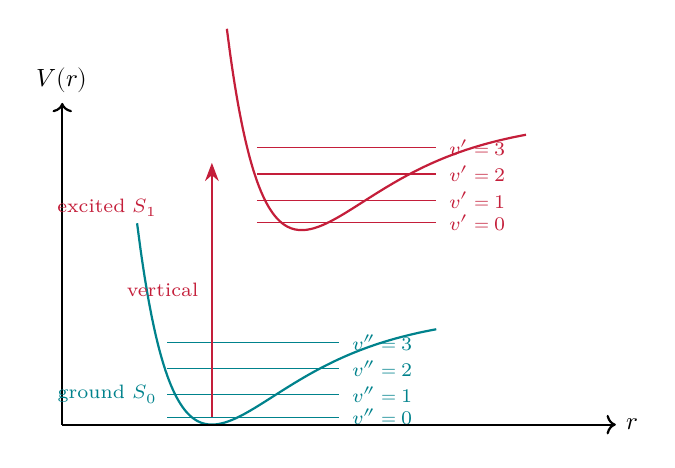
\begin{tikzpicture}[scale=0.95]
  % Lower state Morse
  \draw[myteal, thick, domain=-1.0:3.0, samples=80, smooth, variable=\x] plot ({\x+2.0},{1.5*(1-exp(-0.85*\x))^2});
  % Upper state Morse (shifted right and up)
  \draw[myred, thick, domain=-1.0:3.0, samples=80, smooth, variable=\x] plot ({\x+3.2},{2.6+1.5*(1-exp(-0.85*\x))^2});
  % vibrational levels
  \foreach \v/\y in {0/0.10, 1/0.40, 2/0.75, 3/1.10} {
     \draw[thin, myteal] (1.4,\y) -- (3.7,\y); \node[font=\scriptsize, color=myteal, anchor=west] at (3.75,\y) {$v''=\v$};
  }
  \foreach \v/\y in {0/2.70, 1/3.00, 2/3.35, 3/3.70} {
     \draw[thin, myred] (2.6,\y) -- (5.0,\y);  \node[font=\scriptsize, color=myred, anchor=west] at (5.05,\y) {$v'=\v$};
  }
  % Vertical transition
  \draw[redarrow] (2.0,0.10) -- (2.0,3.50);
  \node[font=\scriptsize, color=myred, anchor=east] at (1.95,1.8) {vertical};
  % axes
  \draw[->, thick] (0,0) -- (7.4,0) node[right, font=\small] {$r$};
  \draw[->, thick] (0,0) -- (0,4.3) node[above, font=\small] {$V(r)$};
  \node[font=\scriptsize, color=myteal] at (0.6,0.4) {ground $S_0$};
  \node[font=\scriptsize, color=myred]  at (0.6,2.9) {excited $S_1$};
\end{tikzpicture}
\end{tcolorbox}

\textbf{Consequences of the Franck--Condon principle:}
\begin{itemize}[leftmargin=*, itemsep=2pt, topsep=2pt]
  \item Absorption spectra of polyatomic molecules show \emph{vibrational fine structure} (a band, not a line).
  \item The most intense vibronic line corresponds to the maximum-overlap (largest Franck--Condon factor) vibrational pair.
  \item After absorption, vibrational relaxation back to $v'=0$ explains the Stokes shift seen in fluorescence.
  \item Combined with Kasha's rule (next sections), it explains why fluorescence emission spectra are wavelength-independent of the excitation $\lambda$.
\end{itemize}

\begin{tcolorbox}[exambox, title={Exam Points (Section 1)}]
\begin{itemize}[leftmargin=*, itemsep=2pt, topsep=2pt]
  \item Always link region of EM spectrum to type of energy: radio--NMR, microwave--rotation, IR--vibration, UV-Vis--electronic.
  \item Use $E=h\nu=hc/\lambda=hc\bar{\nu}$ — examiners love unit conversion problems.
  \item Quote both the gross and specific selection rules; missing the gross rule is the most common cut.
  \item Mutual exclusion principle is a 2-mark gem; remember $\mathrm{CO_2}$.
  \item For NMR sensitivity question, refer to the Boltzmann ratio.
  \item Franck--Condon principle: ``electronic transitions are vertical, nuclei don't move''.
  \item Einstein relation $A_{21}/B_{21}=8\pi h\nu^{3}/c^{3}$ — explains why low-frequency NMR is intrinsically weak.
\end{itemize}
\end{tcolorbox}

% ===============================================================================
\section{Electronic (UV-Visible) Spectroscopy}
% ===============================================================================

\begin{tcolorbox}[defbox]
\textbf{Electronic spectroscopy} (UV-Vis) measures absorption of ultraviolet ($200$--$400\ \mathrm{nm}$) and visible ($400$--$800\ \mathrm{nm}$) light by molecules. The energy is sufficient to promote a valence electron from a filled orbital to an empty higher-energy orbital. The resulting spectrum gives information about chromophores, conjugation, and concentration.
\end{tcolorbox}

\subsection{Types of Electronic Transitions}
The valence electrons of organic molecules occupy four kinds of orbitals: bonding $\sigma$ and $\pi$, non-bonding $n$, and antibonding $\sigma^{*}$ and $\pi^{*}$. The four common electronic transitions, in increasing wavelength (decreasing energy), are listed below.

\begin{tcolorbox}[tikzbox, title={Energy-Level Order of Molecular Orbitals and Possible Transitions}]
\centering
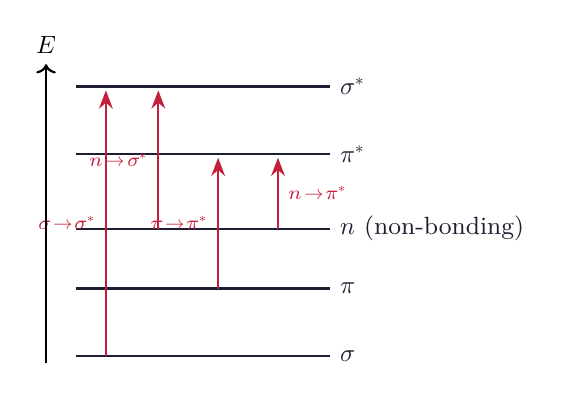
\begin{tikzpicture}[scale=0.95]
  % Levels
  \draw[thick, mydark] (0,0)   -- (3.4,0)   node[right, font=\small] {$\sigma$};
  \draw[thick, mydark] (0,0.9) -- (3.4,0.9) node[right, font=\small] {$\pi$};
  \draw[thick, mydark] (0,1.7) -- (3.4,1.7) node[right, font=\small] {$n$ (non-bonding)};
  \draw[thick, mydark] (0,2.7) -- (3.4,2.7) node[right, font=\small] {$\pi^{*}$};
  \draw[thick, mydark] (0,3.6) -- (3.4,3.6) node[right, font=\small] {$\sigma^{*}$};

  % Transitions (arrows)
  \draw[redarrow] (0.4,0)   -- (0.4,3.55) node[midway, left, font=\scriptsize, color=myred] {$\sigma\!\to\!\sigma^{*}$};
  \draw[redarrow] (1.1,1.7) -- (1.1,3.55) node[midway, left, font=\scriptsize, color=myred] {$n\!\to\!\sigma^{*}$};
  \draw[redarrow] (1.9,0.9) -- (1.9,2.65) node[midway, left, font=\scriptsize, color=myred] {$\pi\!\to\!\pi^{*}$};
  \draw[redarrow] (2.7,1.7) -- (2.7,2.65) node[midway, right, font=\scriptsize, color=myred] {$n\!\to\!\pi^{*}$};

  % Energy axis
  \draw[->, thick] (-0.4,-0.1) -- (-0.4,3.9) node[above, font=\small] {$E$};
\end{tikzpicture}
\end{tcolorbox}

\textbf{Comparison of the four transitions:}\par\noindent
\begin{tabularx}{\linewidth}{|B{2.4cm}|Y|Y|Y|}
\hline
\textbf{Transition} & \textbf{Compounds showing it} & \textbf{$\lambda_{\max}$ region} & \textbf{Intensity ($\varepsilon$)} \\
\hline
$\sigma\!\to\!\sigma^{*}$ & Saturated alkanes (CH$_4$, ethane) & $<150\ \mathrm{nm}$ (vacuum UV) & High but inaccessible \\
\hline
$n\!\to\!\sigma^{*}$ & H$_2$O, CH$_3$OH, alkyl halides, amines & $150$--$250\ \mathrm{nm}$ & Medium ($10^2$--$10^3$) \\
\hline
$\pi\!\to\!\pi^{*}$ & Alkenes, alkynes, aromatics, carbonyls & $170$--$250\ \mathrm{nm}$ & High ($10^3$--$10^4$) \\
\hline
$n\!\to\!\pi^{*}$ & Aldehydes, ketones, $\mathrm{>C{=}O}$, $\mathrm{>C{=}N}$ & $270$--$300\ \mathrm{nm}$ & Low ($10$--$10^2$) \\
\hline
\end{tabularx}

\subsection{Beer--Lambert Law: The Quantitative Backbone}
UV-Vis is a quantitative tool because the absorbance is linearly related to concentration through the Beer--Lambert law.

\begin{tcolorbox}[formulabox, title={Beer--Lambert Law}]
\[
A=\log_{10}\!\frac{I_0}{I}=\varepsilon\,c\,l
\]
\textbf{Symbols:} $A$ = absorbance (dimensionless); $I_0$ = incident intensity; $I$ = transmitted intensity; $\varepsilon$ = molar absorptivity ($\mathrm{L\,mol^{-1}\,cm^{-1}}$); $c$ = concentration ($\mathrm{mol\,L^{-1}}$); $l$ = path length (cm).\\
Also useful:
\[
T=\frac{I}{I_0},\qquad A=-\log_{10}T=2-\log_{10}(\%T)
\]
\end{tcolorbox}

\textbf{Limitations of Beer--Lambert law:}\par\noindent
\begin{tabularx}{\linewidth}{|B{3.4cm}|Y|}
\hline
\textbf{Cause of deviation} & \textbf{Reason} \\
\hline
High concentration ($>10^{-2}\ \mathrm{M}$) & Solute molecules interact, $\varepsilon$ is no longer constant \\
\hline
Polychromatic light & Different wavelengths have different $\varepsilon$, average becomes non-linear \\
\hline
Stray radiation & Light reaching detector by leakage flattens absorbance at high $A$ \\
\hline
Chemical equilibria & Dimerisation, ionisation, fluorescence change effective absorbing species \\
\hline
\end{tabularx}

\begin{tcolorbox}[examplebox, title={Solved Example: Absorbance to Concentration}]
\textbf{Problem:} A solution of an organic dye gives $A=0.92$ in a $1.0\ \mathrm{cm}$ cell at $510\ \mathrm{nm}$, where $\varepsilon=2300\ \mathrm{L\,mol^{-1}\,cm^{-1}}$. Find the concentration.

\textbf{Solution:} From $A=\varepsilon c l$,
\[
c=\frac{A}{\varepsilon l}=\frac{0.92}{2300\times 1.0}=4.0\times 10^{-4}\ \mathrm{mol\,L^{-1}}
\]
\textbf{Exam tip:} Always state whether you used $\log_{10}$ or $\ln$. The IUPAC form uses $\log_{10}$.
\end{tcolorbox}

\subsection{Chromophores and Auxochromes}
Functional groups that determine where a molecule absorbs are called chromophores, while certain saturated groups that shift the band of a chromophore are called auxochromes.

\begin{tcolorbox}[defbox]
\textbf{Chromophore:} Unsaturated functional group responsible for absorption (e.g.\ $\mathrm{C{=}C}$, $\mathrm{C{=}O}$, $\mathrm{N{=}N}$, $\mathrm{NO_2}$).\\
\textbf{Auxochrome:} Saturated group with non-bonding electrons (e.g.\ $\mathrm{-OH}$, $\mathrm{-NH_2}$, $\mathrm{-OR}$, $\mathrm{-X}$) that, when attached to a chromophore, shifts $\lambda_{\max}$ to longer wavelength and increases intensity.
\end{tcolorbox}

\textbf{Standard wavelength-shift terminology:}\par\noindent
\begin{tabularx}{\linewidth}{|B{2.6cm}|Y|Y|}
\hline
\textbf{Term} & \textbf{Effect on $\lambda_{\max}$} & \textbf{Cause} \\
\hline
Bathochromic (red) shift & $\lambda_{\max}$ \emph{increases} & Conjugation, auxochrome, polar solvent (for $\pi\!\to\!\pi^{*}$) \\
\hline
Hypsochromic (blue) shift & $\lambda_{\max}$ \emph{decreases} & Removal of conjugation, polar solvent (for $n\!\to\!\pi^{*}$) \\
\hline
Hyperchromic effect & $\varepsilon$ \emph{increases} & Increased symmetry/conjugation \\
\hline
Hypochromic effect & $\varepsilon$ \emph{decreases} & Distortion of chromophore \\
\hline
\end{tabularx}

\subsection{Effect of Conjugation}
Each additional conjugated $\mathrm{C{=}C}$ raises the highest occupied $\pi$ MO and lowers the lowest empty $\pi^{*}$ MO. The HOMO--LUMO gap shrinks, so $\lambda_{\max}$ moves to longer wavelength.

\begin{tabularx}{\linewidth}{|B{3.0cm}|Y|Y|}
\hline
\textbf{Compound} & \textbf{Conjugated double bonds} & \textbf{$\lambda_{\max}$ (nm)} \\
\hline
Ethylene & 1 & 165 \\
\hline
1,3-Butadiene & 2 & 217 \\
\hline
1,3,5-Hexatriene & 3 & 258 \\
\hline
$\beta$-Carotene & 11 & 470 (orange colour) \\
\hline
\end{tabularx}

\subsection{Solvent Effects on Electronic Spectra}
The solvent stabilises the ground and excited states differently, so the absorption band shifts.

\begin{tabularx}{\linewidth}{|B{2.4cm}|Y|Y|}
\hline
\textbf{Transition} & \textbf{Polar protic solvent effect} & \textbf{Reason} \\
\hline
$\pi\!\to\!\pi^{*}$ & Bathochromic (red shift) & Excited state ($\pi^{*}$) more polar, better stabilised \\
\hline
$n\!\to\!\pi^{*}$ & Hypsochromic (blue shift) & Hydrogen bonds with lone pair lower the ground state more \\
\hline
\end{tabularx}

\subsection{Block Diagram of a UV-Visible Spectrophotometer}
A double-beam spectrophotometer compares the sample beam with a reference beam in real time, eliminating fluctuations of the lamp.

\begin{tcolorbox}[tikzbox, title={Double-Beam UV-Vis Spectrophotometer}]
\centering
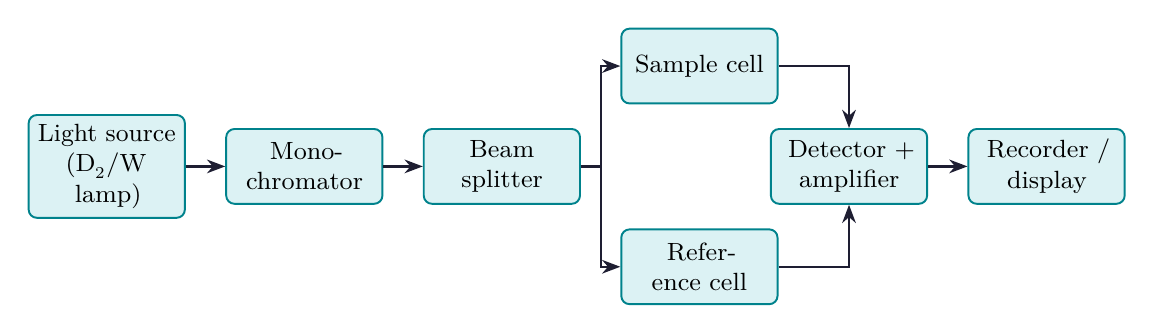
\begin{tikzpicture}[node distance=0.3cm and 0.45cm,
  sblock/.style={rectangle, draw=myteal, fill=hdrteal, text width=1.75cm,
    align=center, minimum height=0.95cm, font=\small,
    rounded corners=3pt, line width=0.7pt}]
  \node[sblock] (n1) {Light source\\(D$_2$/W lamp)};
  \node[sblock, right=0.5cm of n1] (n2) {Mono-chromator};
  \node[sblock, right=0.5cm of n2] (n3) {Beam splitter};
  \node[sblock, above right=0.3cm and 0.5cm of n3] (n4) {Sample cell};
  \node[sblock, below right=0.3cm and 0.5cm of n3] (n5) {Reference cell};
  \node[sblock, right=2.4cm of n3] (n6) {Detector + amplifier};
  \node[sblock, right=0.5cm of n6] (n7) {Recorder /\\display};

  \draw[arrow] (n1) -- (n2);
  \draw[arrow] (n2) -- (n3);
  \draw[arrow] (n3.east) -- ++(0.25,0) |- (n4.west);
  \draw[arrow] (n3.east) -- ++(0.25,0) |- (n5.west);
  \draw[arrow] (n4.east) -| (n6.north);
  \draw[arrow] (n5.east) -| (n6.south);
  \draw[arrow] (n6) -- (n7);
\end{tikzpicture}
\end{tcolorbox}

\textbf{Common light sources and their range:}
\begin{itemize}[leftmargin=*, itemsep=1pt, topsep=2pt]
  \item Deuterium ($\mathrm{D_2}$) lamp — UV region, $190$--$400\ \mathrm{nm}$.
  \item Tungsten--halogen lamp — visible region, $350$--$2500\ \mathrm{nm}$.
  \item Xenon flash lamp — both UV and visible.
\end{itemize}

\subsection{Applications of UV-Visible Spectroscopy}
\begin{itemize}[leftmargin=*, itemsep=2pt, topsep=2pt]
  \item Quantitative estimation of metal ions (Fe$^{3+}$ as thiocyanate, etc.).
  \item Determination of molar absorptivity and concentration in pharmaceuticals.
  \item Detection of conjugated systems and aromatic rings.
  \item Reaction kinetics: change in $A$ with time gives the rate.
  \item Identification of dyes and impurity profiling.
\end{itemize}

\subsection{Woodward--Fieser Rules}
For dienes and $\alpha,\beta$-unsaturated carbonyls, $\lambda_{\max}$ can be predicted to within $\pm 5\ \mathrm{nm}$ by adding empirical increments to a base value. This is a MAKAUT favourite for 5- and 10-mark questions.

\begin{tcolorbox}[formulabox, title={Woodward--Fieser Rule for Dienes}]
\[
\lambda_{\max} = \lambda_{\mathrm{base}} + \sum (\text{increments})
\]
Base values (in nm):\\[2pt]
Acyclic / heteroannular diene: $\bf 215$ \quad Homoannular diene: $\bf 253$\\[6pt]
Common increments:
\begin{itemize}[leftmargin=*, itemsep=1pt, topsep=2pt]
  \item Each extra conjugated $\mathrm{C{=}C}$: $+30$
  \item Alkyl group / ring residue: $+5$
  \item Exocyclic double bond: $+5$
  \item $-\mathrm{OR}$: $+6$, $-\mathrm{OAc}$: $0$, $-\mathrm{Cl}/-\mathrm{Br}$: $+5$, $-\mathrm{NR_2}$: $+60$
\end{itemize}
\end{tcolorbox}

\begin{tcolorbox}[examplebox, title={Solved Example: Predicting \texorpdfstring{$\lambda_{\max}$}{lambda max} of 2,4-Dimethyl-1,3-pentadiene}]
\textbf{Structure:} acyclic diene with two methyl substituents and one ring residue.

\textbf{Calculation:}
\begin{itemize}[leftmargin=*, itemsep=1pt, topsep=2pt]
  \item Base value (acyclic diene) \dotfill $215$
  \item Three alkyl groups $\times +5$ \dotfill $+15$
\end{itemize}
\[
\lambda_{\max}^{\text{pred}} = 215 + 15 = 230\ \mathrm{nm}
\]
\textbf{Reported:} $\lambda_{\max}=232\ \mathrm{nm}$ — within the $\pm 5\ \mathrm{nm}$ rule.
\end{tcolorbox}

\textbf{Woodward--Fieser rule for enones:} The rule extends to $\alpha,\beta$-unsaturated ketones with base value $215\ \mathrm{nm}$ (acyclic / six-ring) and base value $202\ \mathrm{nm}$ (five-ring). Each $\alpha$-substituent adds $10\ \mathrm{nm}$, $\beta$-substituent adds $12\ \mathrm{nm}$, and so on. Beyond the engineering syllabus the principle is the same — pile up empirical increments on a base.

\subsection{Isosbestic Point}
When two species $A$ and $B$ inter-convert (e.g.\ acid--base equilibrium or a kinetic transformation), their UV-Vis spectra cross at one or more wavelengths where the absorbance does \emph{not} change with composition.

\begin{tcolorbox}[defbox]
\textbf{Isosbestic point:} A wavelength at which two absorbing species have the same molar absorptivity. The presence of a sharp isosbestic point in a series of recorded spectra is direct evidence of a clean two-component equilibrium without any third absorbing intermediate.
\end{tcolorbox}

\textbf{Why exam-relevant:} In titrations, kinetic studies, and pH-dependent measurements the isosbestic point lets you measure total concentration independent of the equilibrium position.

\subsection{Single-Beam vs Double-Beam Instruments}
\begin{tabularx}{\linewidth}{|B{2.6cm}|Y|Y|}
\hline
\textbf{Feature} & \textbf{Single-beam} & \textbf{Double-beam} \\
\hline
Light path & One path: source $\to$ sample $\to$ detector & Two paths simultaneously: sample and reference \\
\hline
Reference correction & Manual (run blank, then sample) & Automatic, real-time \\
\hline
Lamp drift & Affects reading & Cancelled out \\
\hline
Cost & Cheaper, simpler & More expensive but more accurate \\
\hline
Use case & Routine fixed-$\lambda$ measurements & Spectral scanning, kinetics \\
\hline
\end{tabularx}

\subsection{Sample Cell (Cuvette) Materials}
Choosing the wrong cuvette is the most common practical mistake — quartz absorbs nothing in UV, glass cuts off below $340\ \mathrm{nm}$.

\begin{tabularx}{\linewidth}{|B{2.6cm}|Y|Y|}
\hline
\textbf{Material} & \textbf{Useful range} & \textbf{Notes} \\
\hline
Quartz / fused silica & $190$--$2500\ \mathrm{nm}$ & Mandatory for UV; expensive \\
\hline
Borosilicate glass & $340$--$2500\ \mathrm{nm}$ & Visible/NIR only \\
\hline
Polystyrene (disposable) & $340$--$800\ \mathrm{nm}$ & Single-use, cheap, visible only \\
\hline
$\mathrm{CaF_2}$ / $\mathrm{BaF_2}$ & $150\ \mathrm{nm}$--mid-IR & Vacuum-UV and IR work \\
\hline
\end{tabularx}

\begin{tcolorbox}[exambox, title={Exam Points (Section 2)}]
\begin{itemize}[leftmargin=*, itemsep=2pt, topsep=2pt]
  \item State all four transitions with energy order: $n\!\to\!\pi^{*}<\pi\!\to\!\pi^{*}<n\!\to\!\sigma^{*}<\sigma\!\to\!\sigma^{*}$.
  \item For Beer--Lambert numericals, watch units of $c$ and $l$.
  \item Always link conjugation with bathochromic shift ($\beta$-carotene, lycopene).
  \item Mention deuterium lamp for UV and tungsten lamp for visible.
  \item Use the Woodward--Fieser increment formula for enone / diene predictions.
  \item Quartz cuvette below $340\ \mathrm{nm}$, glass above $340\ \mathrm{nm}$.
  \item Sharp isosbestic point $=$ clean two-component equilibrium.
\end{itemize}
\end{tcolorbox}

% ===============================================================================
\section{Fluorescence and Its Applications in Medicine}
% ===============================================================================

\begin{tcolorbox}[defbox]
\textbf{Fluorescence} is the spontaneous emission of light by a molecule that has been excited to a higher singlet electronic state, when it returns to its ground state \emph{without changing spin multiplicity}. The emission lifetime is short ($10^{-9}$--$10^{-7}\ \mathrm{s}$), and the emission stops as soon as the exciting source is turned off.
\end{tcolorbox}

\subsection{Singlet, Triplet and the Jablonski Diagram}
A molecule can have its electron pair with antiparallel spins (singlet, $S$) or parallel spins (triplet, $T$). All photophysical processes can be summarised in a Jablonski diagram.

\begin{tcolorbox}[tikzbox, title={Jablonski Energy-Level Diagram}]
\centering
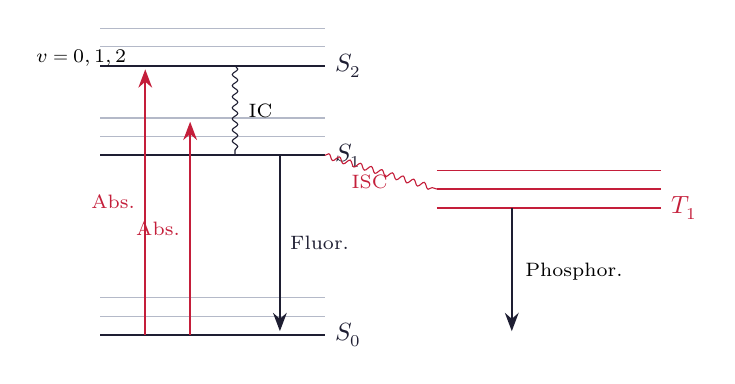
\begin{tikzpicture}[scale=0.95]
  % Singlet manifolds
  \draw[thick, mydark] (0,0) -- (3.0,0)   node[right, font=\small] {$S_0$};
  \draw[thick, mydark] (0,2.4) -- (3.0,2.4) node[right, font=\small] {$S_1$};
  \draw[thick, mydark] (0,3.6) -- (3.0,3.6) node[right, font=\small] {$S_2$};
  % Vibrational sub-levels
  \foreach \y in {0.25, 0.5}  \draw[thin, mgframe] (0,\y) -- (3.0,\y);
  \foreach \y in {2.65, 2.9} \draw[thin, mgframe] (0,\y) -- (3.0,\y);
  \foreach \y in {3.85, 4.1} \draw[thin, mgframe] (0,\y) -- (3.0,\y);
  % Triplet
  \draw[thick, myred] (4.5,1.7) -- (7.5,1.7) node[right, font=\small, color=myred] {$T_1$};
  \foreach \y in {1.95, 2.2} \draw[thin, myred] (4.5,\y) -- (7.5,\y);

  % Absorption arrows
  \draw[redarrow] (0.6,0)   -- (0.6,3.55) node[midway, left, font=\scriptsize, color=myred] {Abs.};
  \draw[redarrow] (1.2,0)   -- (1.2,2.85) node[midway, left, font=\scriptsize, color=myred] {Abs.};

  % IC (internal conversion) wavy down
  \draw[decorate, decoration={snake, amplitude=1pt, segment length=4pt}, color=mydark]
       (1.8,3.6) -- (1.8,2.4);
  \node[font=\scriptsize, anchor=west] at (1.85,3.0) {IC};

  % Fluorescence
  \draw[arrow] (2.4,2.4) -- (2.4,0.05) node[midway, right, font=\scriptsize] {Fluor.};

  % Inter-system crossing
  \draw[decorate, decoration={snake, amplitude=1pt, segment length=4pt}, color=myred]
       (3.0,2.4) -- (4.5,1.95);
  \node[font=\scriptsize, color=myred] at (3.6,2.05) {ISC};

  % Phosphorescence
  \draw[arrow] (5.5,1.7) -- (5.5,0.05);
  \node[font=\scriptsize, anchor=west] at (5.55,0.85) {Phosphor.};

  % Vibrational relaxation labels
  \node[font=\scriptsize] at (-0.25,3.7) {$v=0,1,2$};
\end{tikzpicture}
\end{tcolorbox}

\textbf{Key processes shown in the Jablonski diagram:}
\begin{itemize}[leftmargin=*, itemsep=2pt, topsep=2pt]
  \item \textbf{Absorption}: $S_0\to S_1$ or $S_0\to S_2$ in $10^{-15}\ \mathrm{s}$.
  \item \textbf{Vibrational relaxation (VR)}: loss of excess vibrational energy in $10^{-12}\ \mathrm{s}$.
  \item \textbf{Internal conversion (IC)}: non-radiative $S_2\to S_1$, same multiplicity.
  \item \textbf{Fluorescence (F)}: radiative $S_1\to S_0$ in $10^{-9}$--$10^{-7}\ \mathrm{s}$.
  \item \textbf{Inter-system crossing (ISC)}: $S_1\to T_1$, spin-forbidden but possible.
  \item \textbf{Phosphorescence (P)}: radiative $T_1\to S_0$ in $10^{-3}$--$10\ \mathrm{s}$.
\end{itemize}

\subsection{Fluorescence vs Phosphorescence}
\begin{tabularx}{\linewidth}{|B{3.0cm}|Y|Y|}
\hline
\textbf{Property} & \textbf{Fluorescence} & \textbf{Phosphorescence} \\
\hline
Initial state & Singlet excited ($S_1$) & Triplet excited ($T_1$) \\
\hline
Spin change & None (allowed) & Yes (formally forbidden) \\
\hline
Lifetime & $10^{-9}$--$10^{-7}\ \mathrm{s}$ & $10^{-3}$--$10\ \mathrm{s}$ \\
\hline
After source off & Stops immediately & Persists (afterglow) \\
\hline
Wavelength & Slightly higher than absorption & Even higher than fluorescence \\
\hline
Common at & Room temperature, fluid solution & Low temperature, rigid medium \\
\hline
\end{tabularx}

\subsection{Stokes Shift and Mirror-Image Rule}
\begin{tcolorbox}[defbox]
\textbf{Stokes shift} is the difference between the absorption maximum and the emission maximum, $\Delta\lambda=\lambda_{\mathrm{em}}-\lambda_{\mathrm{abs}}$. It arises because the molecule loses vibrational energy before emitting.\\
\textbf{Mirror-image rule:} For most rigid fluorophores the emission spectrum is approximately a mirror image of the absorption spectrum on the wavelength axis.
\end{tcolorbox}

\subsection{Quantum Yield and Quenching}
\begin{tcolorbox}[formulabox, title={Quantum Yield of Fluorescence}]
\[
\Phi_F=\frac{\text{number of photons emitted}}{\text{number of photons absorbed}}=\frac{k_F}{k_F+k_{NR}+k_{ISC}+k_Q[Q]}
\]
$k_F$ is the radiative rate; $k_{NR}, k_{ISC}, k_Q$ are non-radiative, inter-system crossing and quenching rates respectively. $0\le \Phi_F\le 1$.
\end{tcolorbox}

\textbf{Stern--Volmer equation for collisional quenching:}
\[
\frac{F_0}{F}=1+K_{SV}[Q]
\]
where $F_0$ is fluorescence intensity without quencher, $F$ is intensity in presence of quencher concentration $[Q]$, and $K_{SV}$ is the Stern--Volmer constant.

\subsection{Factors Influencing Fluorescence Intensity}
\begin{tabularx}{\linewidth}{|B{3.4cm}|Y|}
\hline
\textbf{Factor} & \textbf{Effect} \\
\hline
Rigidity of molecule & Rigid planar systems (fluorescein, rhodamine) fluoresce strongly because non-radiative pathways are suppressed. \\
\hline
Conjugation / aromaticity & Extended $\pi$-system shifts emission to longer $\lambda$ and increases $\Phi_F$. \\
\hline
Substituents & Electron-donating ($-\mathrm{NH_2}, -\mathrm{OH}$) enhance; heavy atoms (Br, I) and $\mathrm{NO_2}$ promote ISC and quench. \\
\hline
Solvent & Polar solvent stabilises the more polar excited state $\Rightarrow$ red-shifted, sometimes weaker emission. \\
\hline
Temperature & Higher $T$ increases collisional non-radiative loss $\Rightarrow$ weaker fluorescence. \\
\hline
Dissolved $\mathrm{O_2}$ & Triplet $\mathrm{O_2}$ quenches both fluorescence and phosphorescence. \\
\hline
pH & Protonation/deprotonation of acidic chromophores changes $\Phi_F$ and $\lambda_{em}$. \\
\hline
\end{tabularx}

\subsection{Spectrofluorimeter (Block Diagram)}
A fluorimeter detects light at $90^{\circ}$ to the excitation beam to avoid interference from transmitted light.

\begin{tcolorbox}[tikzbox, title={Block Diagram of a Spectrofluorimeter}]
\centering
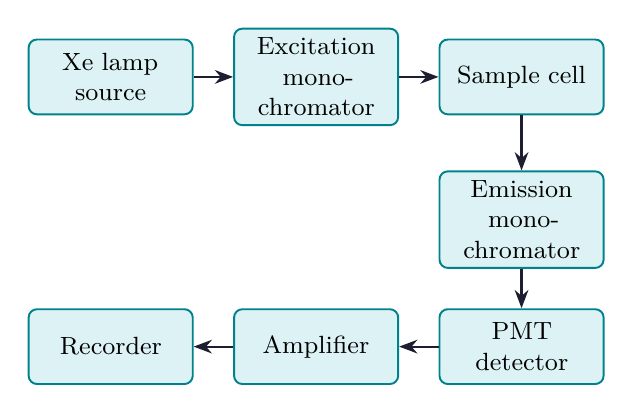
\begin{tikzpicture}[node distance=0.3cm and 0.45cm,
  sblock/.style={rectangle, draw=myteal, fill=hdrteal, text width=1.85cm,
    align=center, minimum height=0.95cm, font=\small,
    rounded corners=3pt, line width=0.7pt}]
  \node[sblock] (lamp) {Xe lamp source};
  \node[sblock, right=0.5cm of lamp] (mono1) {Excitation mono-chromator};
  \node[sblock, right=0.5cm of mono1] (cell) {Sample cell};
  \node[sblock, below=0.7cm of cell] (mono2) {Emission mono-chromator};
  \node[sblock, below=0.5cm of mono2] (det) {PMT detector};
  \node[sblock, left=0.5cm of det] (amp) {Amplifier};
  \node[sblock, left=0.5cm of amp] (rec) {Recorder};

  \draw[arrow] (lamp) -- (mono1);
  \draw[arrow] (mono1) -- (cell);
  \draw[arrow] (cell) -- (mono2);
  \draw[arrow] (mono2) -- (det);
  \draw[arrow] (det) -- (amp);
  \draw[arrow] (amp) -- (rec);
\end{tikzpicture}
\end{tcolorbox}

\subsection{Applications in Medicine and Biology}
Because fluorescence detection can sense single molecules, it has revolutionised diagnostics and therapy. The main medical applications are listed below.

\begin{tabularx}{\linewidth}{|B{3.4cm}|Y|}
\hline
\textbf{Application} & \textbf{How fluorescence is used} \\
\hline
Clinical assays (immunoassay) & Antibodies tagged with fluorescein/rhodamine bind specific antigens; concentration is read from fluorescence intensity (e.g.\ FIA, FACS). \\
\hline
DNA / RNA detection & Intercalating dyes (ethidium bromide, SYBR Green) and fluorescent probes used in gel imaging and \emph{quantitative} real-time PCR. \\
\hline
Fluorescence microscopy & GFP-tagged proteins visualised inside living cells; reveals localisation and dynamics. \\
\hline
Fluorescent angiography & Sodium fluorescein injected intravenously; ophthalmologist captures retinal vasculature images. \\
\hline
Cancer detection / surgery & 5-Aminolaevulinic acid (5-ALA) accumulates as fluorescent protoporphyrin IX in glioma cells; surgeon visualises tumour boundary in blue light. \\
\hline
Photodynamic therapy (PDT) & Light excites a porphyrin photosensitiser; via ISC it generates singlet oxygen which destroys tumour cells. \\
\hline
Pulse oximetry-related & Near-IR fluorescent probes monitor oxygenation; complementary to absorption oximetry. \\
\hline
Drug binding studies & Tryptophan in proteins (intrinsic fluorophore) reports drug-binding through quenching of its $340\ \mathrm{nm}$ band. \\
\hline
Biosensors & Fluorescence quenching of conjugated polymers used in glucose, $\mathrm{Ca^{2+}}$ and pH sensing. \\
\hline
\end{tabularx}

\begin{tcolorbox}[examplebox, title={Solved Example: Stern--Volmer Plot Reading}]
\textbf{Problem:} A fluorescence quenching experiment gives the following data:
\[
[Q] = 0,\,1,\,2\,\mathrm{mM};\quad F = 100,\,67,\,50\ \text{(arb.)}
\]
Find $K_{SV}$.

\textbf{Solution:} Compute $F_0/F$ for each $[Q]$:
\[
F_0/F = 1.00,\,1.49,\,2.00 \ \Rightarrow\ \text{slope}\approx 0.5\ \mathrm{mM^{-1}}
\]
\[
K_{SV}=500\ \mathrm{M^{-1}}
\]
A linear plot confirms purely collisional (dynamic) quenching.
\end{tcolorbox}

\begin{tcolorbox}[masonbox, title={Why Heavy Atoms and Oxygen Quench Fluorescence}]
Heavy atoms (Br, I) and dissolved $\mathrm{O_2}$ promote inter-system crossing $S_1\to T_1$. Once a molecule is in the triplet state, fluorescence is no longer possible. This ``heavy-atom effect'' is the basis of phosphorescent compounds, and the reason why deoxygenation is needed for high-quantum-yield emission measurements.
\end{tcolorbox}

\subsection{Kasha's Rule}
\begin{tcolorbox}[defbox]
\textbf{Kasha's rule:} Emission (fluorescence or phosphorescence) almost always occurs from the \emph{lowest} excited state of a given multiplicity, regardless of which higher state was initially populated by the absorbed photon.
\end{tcolorbox}

\textbf{Why it matters:}
\begin{itemize}[leftmargin=*, itemsep=2pt, topsep=2pt]
  \item Internal conversion $S_n \to S_1$ is much faster than $S_1 \to S_0$ fluorescence.
  \item The fluorescence wavelength is therefore independent of the excitation wavelength.
  \item This is why an excitation spectrum (intensity vs $\lambda_{\mathrm{exc}}$) reproduces the absorption spectrum exactly.
  \item Combined with the Franck--Condon principle (Section 1.7), it gives the mirror-image rule.
\end{itemize}

\subsection{Lifetime, Quantum Yield, and Radiative Rate}
The radiative lifetime $\tau_F$ and quantum yield $\Phi_F$ are not independent — they jointly fix the natural radiative rate $k_F$.

\begin{tcolorbox}[formulabox, title={Lifetime--Quantum Yield Connection}]
\[
\tau_F=\frac{1}{k_F+k_{NR}+k_{ISC}}, \qquad \Phi_F=k_F\,\tau_F
\]
The natural (radiative) lifetime is $\tau_0=1/k_F=\tau_F/\Phi_F$.\\
A short measured $\tau_F$ together with low $\Phi_F$ indicates strong non-radiative deactivation.
\end{tcolorbox}

\textbf{Diagnostic use:} Time-resolved fluorimetry measures $\tau_F$ directly. Combined with the steady-state $\Phi_F$, you can separate radiative ($k_F$) from non-radiative ($k_{NR}+k_{ISC}$) contributions and identify the dominant decay pathway.

\subsection{F\"orster Resonance Energy Transfer (FRET)}
FRET is non-radiative dipole--dipole energy transfer from an excited donor (D$^{*}$) to a nearby ground-state acceptor (A). The efficiency depends very strongly on the donor--acceptor distance, making FRET a ``spectroscopic ruler'' on the $1$--$10\ \mathrm{nm}$ scale.

\begin{tcolorbox}[formulabox, title={FRET Efficiency}]
\[
E=\frac{R_0^{6}}{R_0^{6}+r^{6}}=1-\frac{\tau_{DA}}{\tau_D}
\]
$r$ = donor--acceptor distance; $R_0$ = F\"orster radius (typically $1$--$10\ \mathrm{nm}$, the distance at which $E=50\%$); $\tau_D$ and $\tau_{DA}$ are donor lifetimes alone and in presence of acceptor.\\
Conditions: spectral overlap of donor emission and acceptor absorption; favourable orientation; $r$ within $\sim 2 R_0$.
\end{tcolorbox}

\begin{tcolorbox}[tikzbox, title={FRET: Donor and Acceptor Spectral Overlap}]
\centering
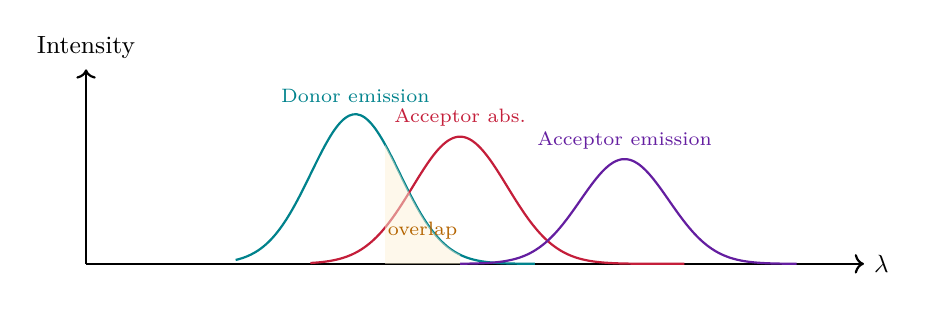
\begin{tikzpicture}[scale=0.95]
  \draw[->, thick] (0,0) -- (10.4,0) node[right, font=\small] {$\lambda$};
  \draw[->, thick] (0,0) -- (0,2.6) node[above, font=\small] {Intensity};
  % Donor emission (teal)
  \draw[myteal, thick, domain=2:6, samples=80, smooth, variable=\x] plot ({\x},{2.0*exp(-((\x-3.6)^2)/0.7)});
  \node[font=\scriptsize, color=myteal] at (3.6,2.25) {Donor emission};
  % Acceptor absorption (red, overlapping)
  \draw[myred, thick, domain=3:8, samples=80, smooth, variable=\x] plot ({\x},{1.7*exp(-((\x-5.0)^2)/0.8)});
  \node[font=\scriptsize, color=myred] at (5.0,1.95) {Acceptor abs.};
  % Acceptor emission (purple, far right)
  \draw[mypurple, thick, domain=5:9.5, samples=80, smooth, variable=\x] plot ({\x},{1.4*exp(-((\x-7.2)^2)/0.7)});
  \node[font=\scriptsize, color=mypurple] at (7.2,1.65) {Acceptor emission};
  % Overlap shading
  \fill[hdramber, opacity=0.5, domain=4:5, variable=\x]
       plot ({\x},{2.0*exp(-((\x-3.6)^2)/0.7)}) -- (5,0) -- (4,0) -- cycle;
  \node[font=\scriptsize, color=myamber] at (4.5,0.45) {overlap};
\end{tikzpicture}
\end{tcolorbox}

\textbf{Medical and biological applications of FRET:}
\begin{itemize}[leftmargin=*, itemsep=1pt, topsep=2pt]
  \item Protein conformational changes (label two residues with D and A).
  \item DNA hybridisation assays and SNP detection.
  \item Real-time PCR with TaqMan probes.
  \item Single-molecule FRET to track folding/binding kinetics.
  \item Fluorescent biosensors for $\mathrm{Ca^{2+}}$, $\mathrm{Zn^{2+}}$, ATP, kinase activity.
\end{itemize}

\begin{tcolorbox}[exambox, title={Exam Points (Section 3)}]
\begin{itemize}[leftmargin=*, itemsep=2pt, topsep=2pt]
  \item Always draw the Jablonski diagram first; mark $S_0, S_1, T_1$, IC, ISC, F, P.
  \item Stokes shift = ``vibrational relaxation before emission''.
  \item Compare F and P using a 4-row table.
  \item Medicine answer must include \emph{at least three} applications: fluorescein angiography, PDT, FIA.
  \item State Kasha's rule and link it to the wavelength-independence of emission.
  \item FRET efficiency $E = R_0^6/(R_0^6+r^6)$ — the $r^{-6}$ distance dependence is the standard 5-mark question.
\end{itemize}
\end{tcolorbox}

% ===============================================================================
\section{Vibrational and Rotational Spectroscopy of Diatomic Molecules}
% ===============================================================================

\begin{tcolorbox}[defbox]
A diatomic molecule rotates about its centre of mass and vibrates along its bond. Photon absorption in the microwave region excites pure rotation; absorption in the infrared region excites vibration (often together with simultaneous rotational changes). Together these tell us bond length, bond strength, force constant, and moment of inertia.
\end{tcolorbox}

\subsection{Rotational Spectroscopy: The Rigid-Rotor Model}
The molecule is modelled as two masses $m_1$ and $m_2$ joined by a rigid rod of length $r$ (the bond length). The reduced mass is
\[
\mu=\frac{m_1 m_2}{m_1+m_2}
\]
and the moment of inertia about the centre of mass is
\[
I=\mu r^{2}
\]

\begin{tcolorbox}[formulabox, title={Rotational Energy Levels (Rigid Rotor)}]
\[
E_J = \frac{\hbar^{2}}{2I}\,J(J+1) \quad\text{or}\quad \tilde{E}_J=\bar{B}\,J(J+1)\ \mathrm{cm^{-1}}
\]
where $J=0,1,2,\ldots$ is the rotational quantum number and the rotational constant is
\[
\bar{B}=\frac{h}{8\pi^{2} c\, I}\ \mathrm{cm^{-1}}
\]
\textbf{Selection rule:} $\Delta J=\pm 1$, and the molecule must possess a permanent dipole moment.
\end{tcolorbox}

\textbf{Spacing of allowed transitions:} For absorption $J\to J+1$,
\[
\Delta\tilde{E}=\tilde{E}_{J+1}-\tilde{E}_{J}=2\bar{B}(J+1)
\]
so successive lines are separated by a constant $2\bar{B}$. From this spacing one can compute $I$, then $r$.

\begin{tcolorbox}[tikzbox, title={Rotational Energy Levels and Spectrum}]
\centering
\begin{tikzpicture}[scale=0.95]
  % Energy ladder
  \foreach \J/\y in {0/0, 1/0.4, 2/1.2, 3/2.4, 4/4.0} {
     \draw[thick, mydark] (0,\y) -- (3.0,\y) node[right, font=\scriptsize] {$J=\J$};
  }
  % Transitions
  \draw[redarrow] (0.4,0)   -- (0.4,0.38);
  \draw[redarrow] (0.9,0.4) -- (0.9,1.18);
  \draw[redarrow] (1.4,1.2) -- (1.4,2.38);
  \draw[redarrow] (1.9,2.4) -- (1.9,3.98);

  % Stick spectrum on right
  \draw[->, thick] (4.6,0) -- (10.6,0) node[right, font=\small] {$\bar{\nu}$};
  \foreach \x/\h in {5.4/1.0, 6.4/1.0, 7.4/1.0, 8.4/1.0, 9.4/1.0} \draw[thick, myteal] (\x,0)--(\x,\h);
  \node[font=\scriptsize] at (5.4,-0.35) {$2\bar{B}$};
  \node[font=\scriptsize] at (6.4,-0.35) {$4\bar{B}$};
  \node[font=\scriptsize] at (7.4,-0.35) {$6\bar{B}$};
  \node[font=\scriptsize] at (8.4,-0.35) {$8\bar{B}$};
  \node[font=\scriptsize] at (9.4,-0.35) {$10\bar{B}$};
\end{tikzpicture}
\end{tcolorbox}

\begin{tcolorbox}[examplebox, title={Solved Example: Bond Length of HCl from Rotational Spectrum}]
\textbf{Problem:} For HCl, $\bar{B}=10.59\ \mathrm{cm^{-1}}$. Calculate the H--Cl bond length. Take $\mu_{\mathrm{HCl}}=1.628\times10^{-27}\ \mathrm{kg}$.

\textbf{Solution:} From $\bar{B}=h/(8\pi^{2}cI)$,
\[
I=\frac{h}{8\pi^{2}c\bar{B}}=\frac{6.626\times10^{-34}}{8\pi^{2}\times 3\times10^{10}\times 10.59}=2.64\times10^{-47}\ \mathrm{kg\,m^{2}}
\]
Using $I=\mu r^{2}$,
\[
r=\sqrt{\frac{I}{\mu}}=\sqrt{\frac{2.64\times10^{-47}}{1.628\times10^{-27}}}=1.27\times10^{-10}\ \mathrm{m}=127\ \mathrm{pm}
\]
\textbf{Result:} The H--Cl bond length is $\approx 127\ \mathrm{pm}$.
\end{tcolorbox}

\subsection{Vibrational Spectroscopy: Simple Harmonic Oscillator Model}
For small displacements the bond can be modelled as a Hookean spring with force constant $k$. Its quantised energies are
\[
E_v=\left(v+\tfrac{1}{2}\right)h\nu_0,\quad v=0,1,2,\ldots,\quad \nu_0=\frac{1}{2\pi}\sqrt{\frac{k}{\mu}}
\]
The fundamental absorption is the $v{=}0\to v{=}1$ transition.

\begin{tcolorbox}[formulabox, title={Vibrational Frequency and Wavenumber}]
\[
\bar{\nu}_0=\frac{1}{2\pi c}\sqrt{\frac{k}{\mu}}\ \mathrm{cm^{-1}}
\]
\textbf{Selection rule:} $\Delta v=\pm 1$ for harmonic oscillator (gross rule: vibration must change the dipole moment).\\
\textbf{Zero-point energy:} $E_0=\tfrac12 h\nu_0\neq 0$, even at $0\ \mathrm{K}$.
\end{tcolorbox}

\begin{tcolorbox}[tikzbox, title={Harmonic Oscillator and Anharmonic (Morse) Potential}]
\centering
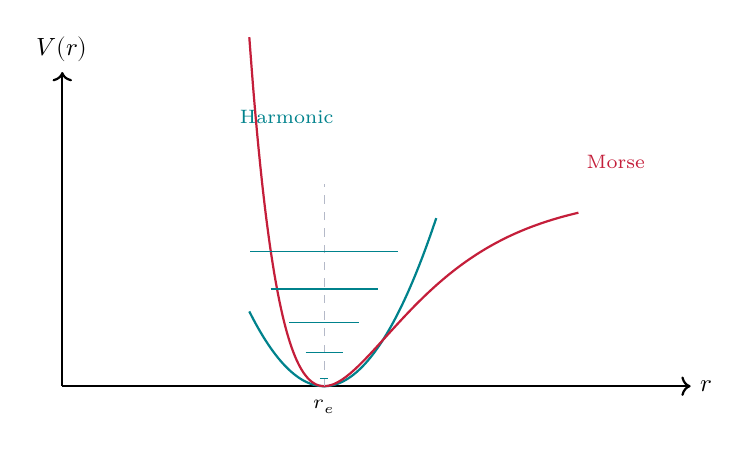
\begin{tikzpicture}[scale=0.95]
  % axes
  \draw[->, thick] (0,0) -- (8.4,0) node[right, font=\small] {$r$};
  \draw[->, thick] (0,0) -- (0,4.2) node[above, font=\small] {$V(r)$};
  % harmonic parabola
  \draw[myteal, thick, domain=-1.0:1.5, samples=80, smooth, variable=\x] plot ({\x+3.5},{(\x)^2});
  \node[font=\scriptsize, color=myteal] at (3.0,3.6) {Harmonic};
  % Morse curve
  \draw[myred, thick, domain=-1.0:3.4, samples=80, smooth, variable=\x] plot ({\x+3.5}, {2.6*(1-exp(-0.85*\x))^2});
  \node[font=\scriptsize, color=myred] at (7.4,3.0) {Morse};
  % equilibrium
  \draw[dashed, mgframe] (3.5,0) -- (3.5,2.7);
  \node[font=\scriptsize, anchor=north] at (3.5,-0.05) {$r_e$};
  % vibrational levels (harmonic)
  \foreach \v/\y in {0/0.10, 1/0.45, 2/0.85, 3/1.30, 4/1.80} {
     \draw[thin, myteal] (3.5-\y*0.55,\y) -- (3.5+\y*0.55,\y);
  }
\end{tikzpicture}
\end{tcolorbox}

\textbf{Anharmonicity (Morse) corrections:}\par\noindent
\begin{tabularx}{\linewidth}{|B{3.6cm}|Y|}
\hline
\textbf{Feature} & \textbf{Effect} \\
\hline
Levels not equally spaced & Spacing decreases as $v$ increases. \\
\hline
Selection rule modified & Overtones $\Delta v=\pm 2,\pm 3,\ldots$ become weakly allowed. \\
\hline
Bond dissociation possible & At sufficient $v$, vibration breaks the bond. \\
\hline
Energy expression & $\tilde{E}_v=\bar{\nu}_e(v+\tfrac12)-\bar{\nu}_e x_e (v+\tfrac12)^{2}$ \\
\hline
\end{tabularx}

\subsection{Vibration--Rotation (Rovibrational) Spectra of Diatomics}
A vibrational transition is usually accompanied by a change in $J$. The fundamental band of HCl, for example, shows a P-branch ($\Delta J=-1$) and an R-branch ($\Delta J=+1$) but \emph{no} central Q-branch ($\Delta J=0$).

\begin{tcolorbox}[tikzbox, title={Rovibrational Spectrum: P and R Branches}]
\centering
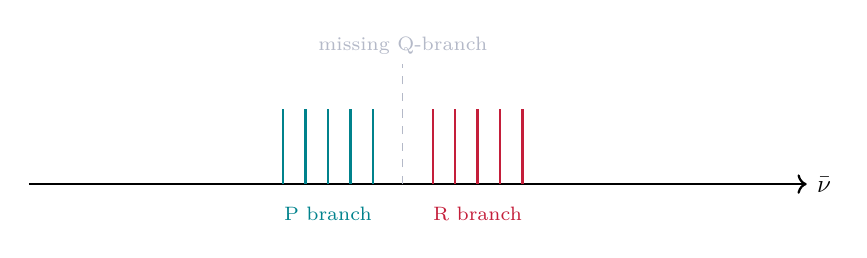
\begin{tikzpicture}[scale=0.95]
  \draw[->, thick] (0,0) -- (10.4,0) node[right, font=\small] {$\bar{\nu}$};
  \draw[dashed, mgframe] (5.0,0) -- (5.0,1.6);
  \node[font=\scriptsize, color=mgframe] at (5.0,1.85) {missing Q-branch};
  % P-branch
  \foreach \x in {3.4, 3.7, 4.0, 4.3, 4.6} \draw[thick, myteal] (\x,0)--(\x,1.0);
  \node[font=\scriptsize, color=myteal] at (4.0,-0.4) {P branch};
  % R-branch
  \foreach \x in {5.4, 5.7, 6.0, 6.3, 6.6} \draw[thick, myred] (\x,0)--(\x,1.0);
  \node[font=\scriptsize, color=myred] at (6.0,-0.4) {R branch};
\end{tikzpicture}
\end{tcolorbox}

\subsection{Modes of Vibration in Polyatomic Molecules}
A non-linear molecule with $N$ atoms has $3N-6$ vibrational modes; a linear one has $3N-5$ modes. Each mode is either stretching (along the bond) or bending (across the bond).

\begin{tcolorbox}[tikzbox, title={Stretching and Bending Vibrations}]
\centering
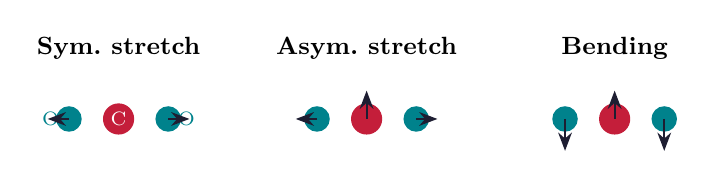
\begin{tikzpicture}[scale=0.9]
  % Symmetric stretch
  \node[font=\small\bfseries] at (1.0,2.0) {Sym.\ stretch};
  \fill[myteal] (0.3,1.0) circle (0.18) node[anchor=east, font=\scriptsize] {O};
  \fill[myred]  (1.0,1.0) circle (0.22) node[font=\scriptsize, color=white] {C};
  \fill[myteal] (1.7,1.0) circle (0.18) node[anchor=west, font=\scriptsize] {O};
  \draw[arrow] (0.3,1.0)--(0.0,1.0);
  \draw[arrow] (1.7,1.0)--(2.0,1.0);

  % Asymmetric stretch
  \node[font=\small\bfseries] at (4.5,2.0) {Asym.\ stretch};
  \fill[myteal] (3.8,1.0) circle (0.18);
  \fill[myred]  (4.5,1.0) circle (0.22);
  \fill[myteal] (5.2,1.0) circle (0.18);
  \draw[arrow] (3.8,1.0)--(3.5,1.0);
  \draw[arrow] (5.2,1.0)--(5.5,1.0);
  \draw[arrow] (4.5,1.0)--(4.5,1.4);

  % Bending
  \node[font=\small\bfseries] at (8.0,2.0) {Bending};
  \fill[myteal] (7.3,1.0) circle (0.18);
  \fill[myred]  (8.0,1.0) circle (0.22);
  \fill[myteal] (8.7,1.0) circle (0.18);
  \draw[arrow] (7.3,1.0)--(7.3,0.55);
  \draw[arrow] (8.7,1.0)--(8.7,0.55);
  \draw[arrow] (8.0,1.0)--(8.0,1.4);
\end{tikzpicture}
\end{tcolorbox}

\textbf{Number of modes for common molecules:}\par\noindent
\begin{tabularx}{\linewidth}{|B{2.6cm}|Y|Y|Y|}
\hline
\textbf{Molecule} & \textbf{Geometry} & \textbf{$3N-5$ or $3N-6$} & \textbf{Modes} \\
\hline
$\mathrm{CO_2}$ & Linear & $3(3)-5$ & 4 (sym str, asym str, two bends) \\
\hline
$\mathrm{H_2O}$ & Bent & $3(3)-6$ & 3 (sym str, asym str, scissor) \\
\hline
$\mathrm{NH_3}$ & Pyramidal & $3(4)-6$ & 6 \\
\hline
$\mathrm{CH_4}$ & Tetrahedral & $3(5)-6$ & 9 \\
\hline
\end{tabularx}

\subsection{Characteristic IR Group Frequencies}
A practical IR fingerprint table is essential for compound identification.

\begin{tabularx}{\linewidth}{|B{3.4cm}|Y|Y|}
\hline
\textbf{Group} & \textbf{Wavenumber (cm$^{-1}$)} & \textbf{Intensity / nature} \\
\hline
O--H (alcohol) & $3200$--$3550$ (broad) & Strong, broad due to H-bond \\
\hline
N--H (amine) & $3300$--$3500$ & Medium, sharp \\
\hline
C--H (sp$^{3}$) & $2850$--$2960$ & Strong \\
\hline
C--H (sp$^{2}$, aromatic) & $3000$--$3100$ & Medium \\
\hline
C${\equiv}$N & $2210$--$2260$ & Medium \\
\hline
C${\equiv}$C & $2100$--$2260$ & Weak \\
\hline
C${=}$O (ester, ketone) & $1680$--$1750$ & Very strong \\
\hline
C${=}$C & $1620$--$1680$ & Variable \\
\hline
N--O (NO$_2$) & $1300$--$1550$ (two bands) & Strong \\
\hline
C--O & $1000$--$1300$ & Strong \\
\hline
\end{tabularx}

\subsection{Block Diagram of an FT-IR Spectrometer}
Modern IR instruments use a Michelson interferometer and Fourier transform of the interferogram to obtain the spectrum.

\begin{tcolorbox}[tikzbox, title={Block Diagram of an FT-IR Spectrometer}]
\centering
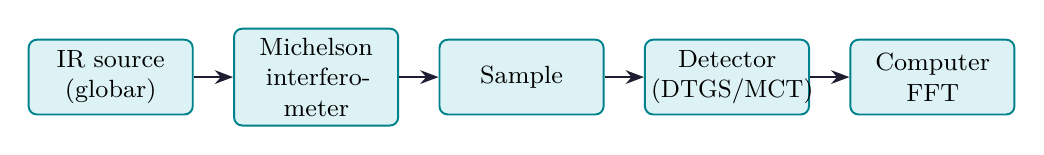
\begin{tikzpicture}[node distance=0.3cm and 0.45cm,
  sblock/.style={rectangle, draw=myteal, fill=hdrteal, text width=1.85cm,
    align=center, minimum height=0.95cm, font=\small,
    rounded corners=3pt, line width=0.7pt}]
  \node[sblock] (n1) {IR source\\(globar)};
  \node[sblock, right=0.5cm of n1] (n2) {Michelson interfero-meter};
  \node[sblock, right=0.5cm of n2] (n3) {Sample};
  \node[sblock, right=0.5cm of n3] (n4) {Detector\\(DTGS/MCT)};
  \node[sblock, right=0.5cm of n4] (n5) {Computer\\FFT};
  \draw[arrow] (n1)--(n2);
  \draw[arrow] (n2)--(n3);
  \draw[arrow] (n3)--(n4);
  \draw[arrow] (n4)--(n5);
\end{tikzpicture}
\end{tcolorbox}

\subsection{Applications of IR and Microwave Spectroscopy}
\begin{itemize}[leftmargin=*, itemsep=2pt, topsep=2pt]
  \item Identification of functional groups (most common organic-chem application).
  \item Distinguishing isomers (e.g.\ acetone vs propanal by C${=}$O stretch position).
  \item Hydrogen bonding studies through O--H shift.
  \item Quantitative analysis using calibrated absorbance.
  \item Microwave spectroscopy gives bond lengths and bond angles to better than $0.1\ \mathrm{pm}$.
  \item Pollution monitoring: IR detects $\mathrm{CO}, \mathrm{CO_2}, \mathrm{NO_x}, \mathrm{SO_2}$ in stack gas.
  \item Polymer/coating analysis (ATR-IR).
\end{itemize}

\subsection{Centrifugal Distortion of the Rigid Rotor}
At higher rotational levels the bond stretches slightly under centrifugal force, increasing the moment of inertia and reducing the spacing between successive lines. The corrected energy expression is
\[
\tilde{E}_J = \bar{B}\,J(J+1) - \bar{D}\,J^{2}(J+1)^{2}
\]
where $\bar{D}$ is the centrifugal-distortion constant ($\bar{D}\ll \bar{B}$). This makes high-$J$ lines slightly closer than the rigid-rotor prediction of $2\bar{B}$ spacing.

\subsection{Isotope Effect on Vibrational and Rotational Spectra}
Replacing $\mathrm{H}$ by $\mathrm{D}$ doubles the reduced mass without changing the force constant. This is a standard MAKAUT viva question and a standard 5-mark numerical.

\begin{tcolorbox}[formulabox, title={Effect of Isotopic Substitution}]
Since $\bar{\nu}_0=(1/2\pi c)\sqrt{k/\mu}$ and $k$ is unchanged,
\[
\frac{\bar{\nu}_{\mathrm{D}}}{\bar{\nu}_{\mathrm{H}}}=\sqrt{\frac{\mu_{\mathrm{H}}}{\mu_{\mathrm{D}}}}\approx \frac{1}{\sqrt{2}}\approx 0.71
\]
For rotational spectra, $\bar{B}\propto 1/\mu r^{2}$, so heavier isotopes give smaller $\bar{B}$ and tighter line spacing.
\end{tcolorbox}

\begin{tcolorbox}[examplebox, title={Solved Example: \texorpdfstring{$\mathrm{H{-}Cl}$}{H-Cl} vs \texorpdfstring{$\mathrm{D{-}Cl}$}{D-Cl} Vibrational Frequency}]
For HCl, $\bar{\nu}_0 \approx 2989\ \mathrm{cm^{-1}}$. Predict $\bar{\nu}_0$ for DCl.\\
The reduced masses are $\mu_{\mathrm{HCl}}=0.972\ \mathrm{u}$ and $\mu_{\mathrm{DCl}}=1.904\ \mathrm{u}$.
\[
\bar{\nu}_{\mathrm{DCl}}=\bar{\nu}_{\mathrm{HCl}}\sqrt{\frac{\mu_{\mathrm{HCl}}}{\mu_{\mathrm{DCl}}}}=2989\sqrt{\frac{0.972}{1.904}}=2989\times 0.715=2137\ \mathrm{cm^{-1}}
\]
Observed value: $2145\ \mathrm{cm^{-1}}$ — excellent agreement.
\end{tcolorbox}

\subsection{Fingerprint Region vs Functional-Group Region}
The IR spectrum is conventionally divided into two regions, and they are used differently in identification.

\begin{tabularx}{\linewidth}{|B{2.8cm}|Y|Y|}
\hline
\textbf{Region} & \textbf{Range (cm$^{-1}$)} & \textbf{Use} \\
\hline
Functional-group region & $4000$--$1500$ & Quick identification of common groups (O--H, N--H, C--H, C${=}$O, C${\equiv}$N, etc.). \\
\hline
Fingerprint region & $1500$--$400$ & Highly specific to the whole molecule; used to confirm identity by comparison with a reference spectrum. Do not assign every peak; match the overall pattern. \\
\hline
\end{tabularx}

\subsection{Sample Preparation for IR Spectroscopy}
The right method depends on the physical state of the sample.

\begin{tabularx}{\linewidth}{|B{2.8cm}|Y|Y|}
\hline
\textbf{Sample} & \textbf{Method} & \textbf{Notes} \\
\hline
Solid (crystalline) & KBr pellet & 1\,\% sample in dry KBr, pressed at $10\ \mathrm{tonnes}$; KBr is IR-transparent above $400\ \mathrm{cm^{-1}}$. \\
\hline
Solid (amorphous) & Nujol mull & Mineral oil paste between two NaCl plates. Nujol bands at $\sim 2900, 1460, 1380\ \mathrm{cm^{-1}}$ — ignore them. \\
\hline
Liquid (neat) & Capillary film & Single drop between two NaCl windows. \\
\hline
Liquid (dilute) & Solution cell & $\mathrm{CCl_4}$, $\mathrm{CHCl_3}$, or $\mathrm{CS_2}$ — all transparent in different ranges. \\
\hline
Gas & Long-path gas cell & $5$--$10\ \mathrm{cm}$ path, NaCl/KBr windows. \\
\hline
Surface / film & ATR (attenuated total reflectance) & No prep needed; press sample on Ge/diamond crystal. \\
\hline
\end{tabularx}

\subsection{IR vs Raman: Side-by-Side Comparison}
\begin{tabularx}{\linewidth}{|B{2.8cm}|Y|Y|}
\hline
\textbf{Feature} & \textbf{IR} & \textbf{Raman} \\
\hline
Photon process & Absorption & Inelastic scattering \\
\hline
Gross selection rule & Vibration must change \emph{dipole} & Vibration must change \emph{polarisability} \\
\hline
Strongest for & Polar bonds (O--H, C${=}$O) & Symmetric, non-polar bonds (C${=}$C, S--S) \\
\hline
Water as solvent & Bad (water absorbs strongly) & Excellent (water is a weak Raman scatterer) \\
\hline
Sample prep & KBr pellet, mull, ATR & Almost none; can be in glass capillary \\
\hline
Source & IR globar & Visible / NIR laser \\
\hline
Sensitivity & High & Low (only $\sim 10^{-7}$ of incident photons scattered) \\
\hline
\end{tabularx}

\begin{tcolorbox}[exambox, title={Exam Points (Section 4)}]
\begin{itemize}[leftmargin=*, itemsep=2pt, topsep=2pt]
  \item Quote both the gross rule (dipole change) and specific rule ($\Delta v=\pm1$) for IR.
  \item For numericals: $\bar{B}=h/(8\pi^{2}cI)$ and $\bar{\nu}_0=(1/2\pi c)\sqrt{k/\mu}$.
  \item Mention zero-point energy as a quantum effect.
  \item For polyatomic, give $3N-6$ / $3N-5$ rule with $\mathrm{H_2O}$/$\mathrm{CO_2}$ example.
  \item Always cite C${=}$O ($\sim 1700\ \mathrm{cm^{-1}}$) and O--H ($\sim 3400\ \mathrm{cm^{-1}}$) bands.
  \item Isotope shift $\bar{\nu}_{\mathrm{D}}/\bar{\nu}_{\mathrm{H}} \approx 1/\sqrt{2}$ for X--H vs X--D — standard 5-mark numerical.
  \item Sample prep choice: KBr pellet for solids, ATR for everything else.
  \item Fingerprint region $<1500\ \mathrm{cm^{-1}}$ confirms identity, functional-group region $>1500\ \mathrm{cm^{-1}}$ identifies groups.
\end{itemize}
\end{tcolorbox}

% ===============================================================================
\section{Nuclear Magnetic Resonance (NMR) and Magnetic Resonance Imaging (MRI)}
% ===============================================================================

\begin{tcolorbox}[defbox]
\textbf{Nuclear Magnetic Resonance (NMR)} is the absorption of radio-frequency radiation by nuclei placed in a strong magnetic field. Only nuclei with non-zero spin quantum number $I\neq 0$ are NMR-active (e.g.\ $^{1}\mathrm{H}, ^{13}\mathrm{C}, ^{19}\mathrm{F}, ^{31}\mathrm{P}$). The chemical environment of each nucleus modifies the resonance frequency and gives a structural fingerprint of the molecule.
\end{tcolorbox}

\subsection{Nuclear Spin and Magnetic Moment}
A nucleus with spin $I$ has a magnetic moment
\[
\vec{\mu}=\gamma\,\vec{I}\,\hbar
\]
where $\gamma$ is the magnetogyric ratio. In an external field $\vec{B}_0$, the spin can take $2I+1$ orientations of energy
\[
E_m=-\gamma m_I\hbar B_0,\qquad m_I=I, I-1,\ldots,-I
\]
For a $^{1}\mathrm{H}$ nucleus ($I=1/2$) only two states exist: $m_I=+1/2$ (lower, aligned with $B_0$) and $m_I=-1/2$ (higher, opposed).

\begin{tcolorbox}[formulabox, title={Larmor (Resonance) Condition}]
\[
\Delta E = \gamma\hbar B_0 = h\nu_L \quad\Rightarrow\quad \nu_L=\frac{\gamma B_0}{2\pi}
\]
$\nu_L$ is called the Larmor frequency. \textbf{Selection rule:} $\Delta m_I=\pm 1$.\\
For $^{1}\mathrm{H}$ in $B_0=11.74\ \mathrm{T}$, $\nu_L=500\ \mathrm{MHz}$.
\end{tcolorbox}

\subsection{Chemical Shift}
The local electron cloud shields each nucleus, so the actual field experienced is $B_{\mathrm{eff}}=B_0(1-\sigma)$, where $\sigma$ is the shielding constant. Different chemical environments have different $\sigma$, leading to slightly different resonance frequencies. To make the values instrument-independent, the chemical shift is referenced to TMS (tetramethylsilane).

\begin{tcolorbox}[formulabox, title={Chemical Shift}]
\[
\delta\ (\mathrm{ppm}) = \frac{\nu_{\mathrm{sample}}-\nu_{\mathrm{TMS}}}{\nu_{\mathrm{spectrometer}}}\times 10^{6}
\]
Higher $\delta$ = deshielded = downfield. Lower $\delta$ = shielded = upfield. TMS is set at $\delta=0\ \mathrm{ppm}$.
\end{tcolorbox}

\textbf{Typical $^{1}\mathrm{H}$ chemical shift ranges:}\par\noindent
\begin{tabularx}{\linewidth}{|B{3.4cm}|Y|Y|}
\hline
\textbf{Type of proton} & \textbf{$\delta$ (ppm)} & \textbf{Comment} \\
\hline
TMS & 0.0 & Reference standard \\
\hline
Alkyl C--H & 0.5--2.0 & Most shielded \\
\hline
Allylic / $\alpha$-carbonyl & 2.0--3.0 & Slight deshielding \\
\hline
$\mathrm{C{-}O{-}H}$, $\mathrm{C{-}O{-}CH}$ & 3.0--4.5 & Deshielded by O \\
\hline
Vinyl ($\mathrm{C{=}CH}$) & 4.5--6.5 & $\pi$-electron shielding \\
\hline
Aromatic & 6.5--8.5 & Ring current deshielding \\
\hline
Aldehyde ($\mathrm{CHO}$) & 9.0--10.0 & Strong deshielding by C${=}$O \\
\hline
Carboxylic acid OH & 10--13 (broad) & H-bonded, broad \\
\hline
\end{tabularx}

\subsection{Spin--Spin Coupling and Multiplicity}
Adjacent magnetic nuclei split each other's signals. The number of equivalent neighbours $n$ produces $n+1$ lines in a binomial intensity ratio (Pascal's triangle).

\begin{tcolorbox}[formulabox, title={\texorpdfstring{$n+1$}{n+1} Rule}]
\[
\text{multiplicity}=n+1
\]
where $n$ is the number of \emph{equivalent} neighbouring (vicinal) protons. The coupling constant $J$ is measured in Hz and is independent of $B_0$.
\end{tcolorbox}

\textbf{Common multiplets:}\par\noindent
\begin{tabularx}{\linewidth}{|B{2.4cm}|Y|Y|Y|}
\hline
\textbf{$n$ neighbours} & \textbf{Pattern} & \textbf{Intensity ratio} & \textbf{Example} \\
\hline
0 & Singlet & 1 & $\mathrm{(CH_3)_4Si}$ \\
\hline
1 & Doublet & 1:1 & CHCl$_2$--CH (coupled to 1H) \\
\hline
2 & Triplet & 1:2:1 & CH$_3$--CH$_2$--X \\
\hline
3 & Quartet & 1:3:3:1 & X--CH$_2$--CH$_3$ \\
\hline
6 & Septet & 1:6:15:20:15:6:1 & Isopropyl CH \\
\hline
\end{tabularx}

\begin{tcolorbox}[examplebox, title={Solved Example: NMR of Ethanol (\texorpdfstring{$\mathrm{CH_3CH_2OH}$}{CH3CH2OH})}]
\textbf{Three sets of equivalent protons:}
\begin{itemize}[leftmargin=*, itemsep=1pt, topsep=2pt]
  \item $\mathrm{CH_3}$ : $\delta\approx 1.2\ \mathrm{ppm}$, \textbf{triplet} (coupled to 2 CH$_2$ neighbours).
  \item $\mathrm{CH_2}$ : $\delta\approx 3.7\ \mathrm{ppm}$, \textbf{quartet} (coupled to 3 CH$_3$ neighbours).
  \item $\mathrm{OH}$ : $\delta\approx 2.6\ \mathrm{ppm}$, broad \textbf{singlet} (rapid exchange averages coupling).
\end{itemize}
Integration ratio: $3:2:1$, exactly matching the proton counts.
\end{tcolorbox}

\subsection{Block Diagram of an NMR Spectrometer}
Modern instruments are pulsed Fourier-transform spectrometers (FT-NMR), which excite all nuclei simultaneously with a strong RF pulse and detect the free-induction decay (FID).

\begin{tcolorbox}[tikzbox, title={Block Diagram of FT-NMR}]
\centering
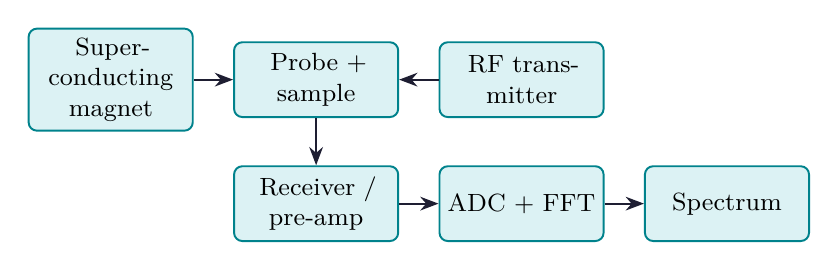
\begin{tikzpicture}[node distance=0.3cm and 0.45cm,
  sblock/.style={rectangle, draw=myteal, fill=hdrteal, text width=1.85cm,
    align=center, minimum height=0.95cm, font=\small,
    rounded corners=3pt, line width=0.7pt}]
  \node[sblock] (mag)  {Super-conducting magnet};
  \node[sblock, right=0.5cm of mag]  (probe) {Probe + sample};
  \node[sblock, right=0.5cm of probe] (rf)   {RF transmitter};
  \node[sblock, below=0.6cm of probe] (rec)  {Receiver / pre-amp};
  \node[sblock, right=0.5cm of rec]  (adc)  {ADC + FFT};
  \node[sblock, right=0.5cm of adc]  (disp) {Spectrum};
  \draw[arrow] (rf) -- (probe);
  \draw[arrow] (mag) -- (probe);
  \draw[arrow] (probe) -- (rec);
  \draw[arrow] (rec) -- (adc);
  \draw[arrow] (adc) -- (disp);
\end{tikzpicture}
\end{tcolorbox}

\subsection{Applications of NMR}
\begin{itemize}[leftmargin=*, itemsep=2pt, topsep=2pt]
  \item Structural elucidation of organic compounds (number of H environments, connectivity, stereochemistry).
  \item Molecular dynamics: relaxation times $T_1$ and $T_2$ probe motion.
  \item Quantitative NMR (qNMR) for drug purity certification.
  \item Solid-state NMR (MAS) for polymers, batteries, and materials.
  \item Protein structure determination via 2D NOESY/HSQC.
\end{itemize}

\subsection{Magnetic Resonance Imaging (MRI)}
MRI applies the principles of NMR to image the inside of the human body without ionising radiation.

\begin{tcolorbox}[defbox]
\textbf{MRI} produces tomographic images by spatially encoding the NMR signal of water protons in the body using \emph{magnetic field gradients}, then reconstructing the image by Fourier transform.
\end{tcolorbox}

\textbf{Why protons?} The body contains $\sim 60$--$70\%$ water, providing an abundant $^{1}\mathrm{H}$ signal. Different tissues differ in (i) proton density, (ii) longitudinal relaxation time $T_1$, and (iii) transverse relaxation time $T_2$ — the key contrast parameters.

\begin{tcolorbox}[formulabox, title={Spatial Encoding using Gradient Fields}]
A linear gradient $G_z=\partial B/\partial z$ makes the resonance frequency of a proton depend on its position $z$:
\[
\nu(z)=\frac{\gamma}{2\pi}\,\bigl(B_0 + G_z\,z\bigr)
\]
Combining $x, y, z$ gradients with phase and frequency encoding produces a 2D or 3D image.
\end{tcolorbox}

\begin{tcolorbox}[tikzbox, title={Major Components of an MRI Scanner}]
\centering
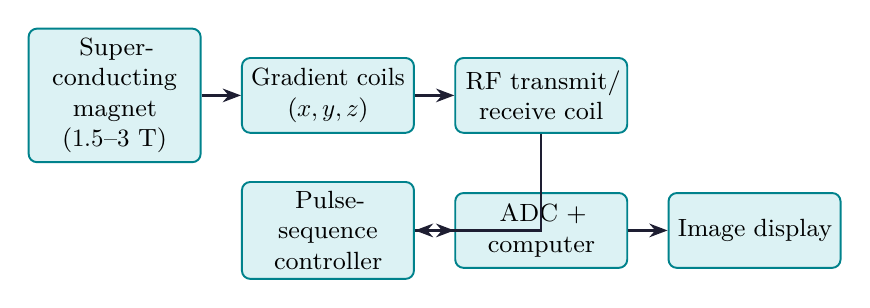
\begin{tikzpicture}[node distance=0.3cm and 0.45cm,
  sblock/.style={rectangle, draw=myteal, fill=hdrteal, text width=1.95cm,
    align=center, minimum height=0.95cm, font=\small,
    rounded corners=3pt, line width=0.7pt}]
  \node[sblock] (n1) {Super-conducting magnet ($1.5$--$3\ \mathrm{T}$)};
  \node[sblock, right=0.5cm of n1] (n2) {Gradient coils\\($x,y,z$)};
  \node[sblock, right=0.5cm of n2] (n3) {RF transmit/ receive coil};
  \node[sblock, below=0.6cm of n2] (n4) {Pulse-sequence controller};
  \node[sblock, right=0.5cm of n4] (n5) {ADC +\\computer};
  \node[sblock, right=0.5cm of n5] (n6) {Image display};
  \draw[arrow] (n1)--(n2);
  \draw[arrow] (n2)--(n3);
  \draw[arrow] (n3) |- (n4);
  \draw[arrow] (n4)--(n5);
  \draw[arrow] (n5)--(n6);
\end{tikzpicture}
\end{tcolorbox}

\subsection{T\texorpdfstring{$_1$}{1} and T\texorpdfstring{$_2$}{2} Contrast}
\begin{tabularx}{\linewidth}{|B{3.0cm}|Y|Y|}
\hline
\textbf{Image type} & \textbf{Contrast source} & \textbf{Tissue look} \\
\hline
$T_1$-weighted & Short TR, short TE; differences in spin--lattice relaxation & Fat is bright, water (CSF) is dark \\
\hline
$T_2$-weighted & Long TR, long TE; differences in spin--spin relaxation & Water is bright, fat is intermediate \\
\hline
Proton density & Long TR, short TE & Reflects total $^{1}\mathrm{H}$ count \\
\hline
fMRI (BOLD) & Magnetic susceptibility change of haemoglobin & Detects neural activity \\
\hline
\end{tabularx}

\subsection{Advantages and Limitations of MRI}
\begin{tabularx}{\linewidth}{|B{3.0cm}|Y|Y|}
\hline
\textbf{Aspect} & \textbf{Advantages} & \textbf{Limitations} \\
\hline
Radiation & Non-ionising, safe & --- \\
\hline
Soft-tissue contrast & Excellent (best of all imaging modalities) & --- \\
\hline
Cost & --- & Very expensive scanner and cryogen \\
\hline
Acquisition time & --- & Several minutes per sequence \\
\hline
Patient compatibility & --- & Pacemakers, ferromagnetic implants, claustrophobia \\
\hline
\end{tabularx}

\subsection{Medical Applications of MRI}
\begin{itemize}[leftmargin=*, itemsep=2pt, topsep=2pt]
  \item Brain: tumour detection, multiple sclerosis, stroke (diffusion MRI).
  \item Spinal cord and joints: disc prolapse, ligament tears.
  \item Cardiac MRI: chamber size, ejection fraction, myocardial viability.
  \item Functional MRI (fMRI): mapping of brain activity using BOLD contrast.
  \item Magnetic resonance angiography (MRA) without iodinated contrast.
  \item Whole-body screening and oncology staging.
\end{itemize}

\subsection{Origin of Chemical Shift: Shielding Mechanisms}
A nucleus's resonance frequency is determined by the local field $B_{\mathrm{eff}}=B_0(1-\sigma)$. The shielding constant $\sigma$ has three additive contributions in organic molecules.

\begin{tabularx}{\linewidth}{|B{3.4cm}|Y|}
\hline
\textbf{Mechanism} & \textbf{Effect} \\
\hline
Diamagnetic shielding ($\sigma_d$) & Local circulation of bonding electrons opposes $B_0$. Increases with electron density on the nucleus. Electronegative neighbours \emph{decrease} $\sigma_d$ and shift signal downfield. \\
\hline
Paramagnetic shielding ($\sigma_p$) & Mixing of low-lying excited states with the ground state \emph{adds} to $B_{\mathrm{eff}}$ and shifts signal downfield. Important in $^{13}\mathrm{C}$ but small in $^{1}\mathrm{H}$. \\
\hline
Anisotropic / ring-current shielding & Aromatic $\pi$-electrons circulate in $B_0$, generating a secondary field. Protons \emph{above/below} the ring are shielded; protons \emph{at the edge} are deshielded ($\delta\sim 7$--$8\ \mathrm{ppm}$). \\
\hline
\end{tabularx}

\textbf{Why TMS is the reference:} Si is electropositive, the four equivalent $\mathrm{CH_3}$ groups are heavily shielded (high electron density on H), and TMS has only one sharp singlet at very low $\delta$, well outside the range of typical organic protons. It is also chemically inert, volatile, and miscible with most solvents.

\subsection{Coupling Constant J and Integration}
A $^{1}\mathrm{H}$ NMR spectrum delivers four pieces of information; the multiplet pattern alone is not enough.

\begin{tabularx}{\linewidth}{|B{3.0cm}|Y|}
\hline
\textbf{Information} & \textbf{Reads from} \\
\hline
Chemical environment & Number of separate signals (peaks at different $\delta$). \\
\hline
Chemical shift $\delta$ & Position in ppm; identifies the type of proton. \\
\hline
Coupling pattern & Number of neighbours through $n+1$ rule. \\
\hline
Integration & Area under each peak; ratio gives \emph{number of protons} in each environment. \\
\hline
\end{tabularx}

\begin{tcolorbox}[formulabox, title={Coupling Constant \texorpdfstring{$J$}{J}}]
\[
J\ (\mathrm{Hz}) = (\nu_2 - \nu_1)
\]
$J$ is measured directly from the line spacing within a multiplet and is \emph{independent} of $B_0$ (chemical shift in Hz scales with $B_0$, but $J$ does not). This is the standard way to distinguish a closely-spaced multiplet from two coincidentally overlapping singlets.
\end{tcolorbox}

\textbf{Typical $^{1}\mathrm{H}{-}^{1}\mathrm{H}$ coupling constants:}
\begin{itemize}[leftmargin=*, itemsep=1pt, topsep=2pt]
  \item Geminal ($^{2}J$, on same C): $-12$ to $+15\ \mathrm{Hz}$.
  \item Vicinal ($^{3}J$, on adjacent C, freely rotating): $6$--$8\ \mathrm{Hz}$.
  \item Vicinal cis (alkene): $6$--$12\ \mathrm{Hz}$.
  \item Vicinal trans (alkene): $12$--$18\ \mathrm{Hz}$.
  \item Aromatic ortho: $\sim 8\ \mathrm{Hz}$, meta: $\sim 2\ \mathrm{Hz}$, para: $<1\ \mathrm{Hz}$.
\end{itemize}

\begin{tcolorbox}[examplebox, title={Solved Example: Distinguishing Cis and Trans Alkenes from \texorpdfstring{$J$}{J}}]
\textbf{Problem:} A sample of \emph{butenedioic acid} can be either maleic acid (cis) or fumaric acid (trans). The vinyl proton signals split into two doublets with $J=11.6\ \mathrm{Hz}$.

\textbf{Solution:} $J$ is in the cis range ($6$--$12\ \mathrm{Hz}$), well below the trans range ($12$--$18\ \mathrm{Hz}$). $\Rightarrow$ \textbf{maleic acid} (cis isomer).
\end{tcolorbox}

\subsection{MRI Contrast Agents}
Some pathologies are hard to see in native $T_1$ or $T_2$ contrast. A paramagnetic contrast agent is then injected intravenously to enhance differences locally.

\begin{tabularx}{\linewidth}{|B{2.8cm}|Y|Y|}
\hline
\textbf{Class} & \textbf{Mechanism} & \textbf{Examples} \\
\hline
Gadolinium chelates & $\mathrm{Gd^{3+}}$ has 7 unpaired electrons; shortens water $T_1$, brightens regions where it accumulates & Gd-DTPA (Magnevist), Gd-DOTA (Dotarem) \\
\hline
SPIONs (super-paramagnetic iron oxide nanoparticles) & Strong local field inhomogeneities shorten $T_2$, darken regions where they accumulate & Ferumoxytol, Resovist \\
\hline
Hyperpolarised gases / metabolites & External polarisation amplifies signal of $^{129}\mathrm{Xe}$, $^{13}\mathrm{C}$-pyruvate, etc. & Xe lung MRI, $^{13}\mathrm{C}$ metabolic MRI \\
\hline
\end{tabularx}

\textbf{Safety note:} Free $\mathrm{Gd^{3+}}$ is toxic; clinical agents use a strong chelator (DTPA, DOTA) to keep it bound until the agent is renally excreted. Patients with reduced kidney function (eGFR\,$<30$) avoid Gd contrast due to nephrogenic systemic fibrosis risk.

\begin{tcolorbox}[masonbox, title={Why MRI Has Better Soft-Tissue Contrast than X-ray CT}]
X-ray CT contrast comes only from electron density, so most soft tissues look similar. MRI exploits proton density \emph{and} two relaxation times $T_1, T_2$, giving multiple contrast knobs and clear discrimination of grey vs white matter, oedema vs tumour, etc.
\end{tcolorbox}

\begin{tcolorbox}[exambox, title={Exam Points (Section 5)}]
\begin{itemize}[leftmargin=*, itemsep=2pt, topsep=2pt]
  \item NMR-active nuclei need $I\neq 0$. List $^{1}\mathrm{H}, ^{13}\mathrm{C}, ^{19}\mathrm{F}, ^{31}\mathrm{P}$.
  \item Always quote Larmor equation $\nu=\gamma B_0/2\pi$.
  \item Use the $n+1$ rule and Pascal's triangle to sketch multiplets.
  \item Define $\delta$ in ppm and reference TMS.
  \item For MRI, mention magnetic gradients for spatial encoding and $T_1/T_2$ contrast.
  \item Three shielding mechanisms: diamagnetic, paramagnetic, ring-current.
  \item Coupling constant $J$ is in Hz and \emph{independent} of $B_0$ (chemical shift in Hz is not).
  \item Distinguish cis/trans alkenes from $J$ values: cis $6$--$12\ \mathrm{Hz}$, trans $12$--$18\ \mathrm{Hz}$.
  \item Gd-DTPA shortens water $T_1$ and brightens MRI images; SPIONs shorten $T_2$ and darken them.
\end{itemize}
\end{tcolorbox}

% ===============================================================================
\section{Surface Characterisation Techniques}
% ===============================================================================

\begin{tcolorbox}[defbox]
\textbf{Surface characterisation} techniques probe the outermost few atomic layers of a solid to give information about (i) topography (shape and roughness), (ii) elemental composition, (iii) chemical state of surface atoms, and (iv) electronic structure. They are essential for catalysts, semiconductors, thin films, biomaterials, and corrosion studies.
\end{tcolorbox}

\subsection{Why a Special Technique for Surfaces?}
Bulk techniques (e.g.\ XRD) average over millions of atomic layers and miss surface effects such as adsorption, oxidation, segregation, and reconstruction. Surface techniques use probes (electrons, ions, photons, mechanical tip) that penetrate only a few nanometres.

\begin{tabularx}{\linewidth}{|B{2.6cm}|Y|Y|Y|}
\hline
\textbf{Technique} & \textbf{Probe in} & \textbf{Signal out} & \textbf{Information} \\
\hline
SEM & Electrons (5--30 kV) & Secondary / back-scattered electrons & Topography, morphology \\
\hline
TEM & Electrons (100--300 kV) & Transmitted electrons & Internal structure, lattice imaging \\
\hline
AFM & Sharp tip & Tip deflection / force & Atomic-scale topography \\
\hline
STM & Tunnelling current & Current vs $z$ & Electronic + topographic image \\
\hline
XPS / ESCA & Soft X-rays & Photo-electrons (KE) & Surface composition, oxidation state \\
\hline
AES & Electron beam & Auger electrons & Elemental composition (light elements) \\
\hline
SIMS & Ion beam & Sputtered secondary ions & Trace elements, depth profile \\
\hline
\end{tabularx}

\subsection{Scanning Electron Microscopy (SEM)}
A focused beam of electrons is rastered over the surface; secondary electrons (SE) reveal topography while back-scattered electrons (BSE) give compositional contrast.

\begin{tcolorbox}[tikzbox, title={Block Diagram of an SEM}]
\centering
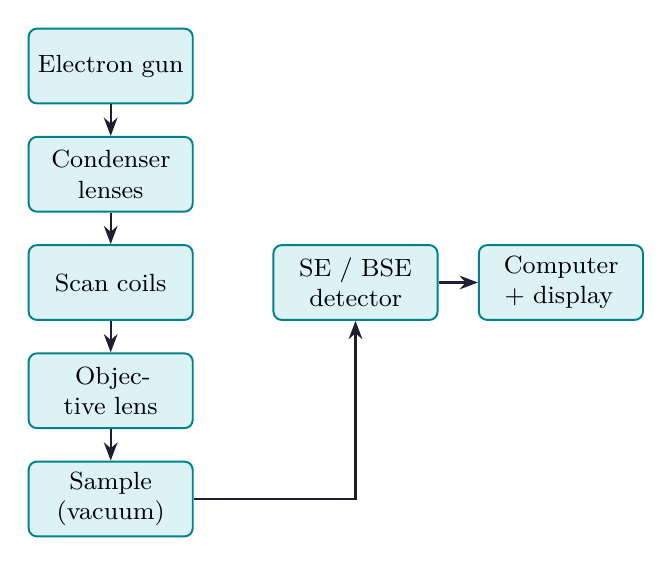
\begin{tikzpicture}[node distance=0.3cm and 0.45cm,
  sblock/.style={rectangle, draw=myteal, fill=hdrteal, text width=1.85cm,
    align=center, minimum height=0.95cm, font=\small,
    rounded corners=3pt, line width=0.7pt}]
  \node[sblock] (n1) {Electron gun};
  \node[sblock, below=0.4cm of n1] (n2) {Condenser lenses};
  \node[sblock, below=0.4cm of n2] (n3) {Scan coils};
  \node[sblock, below=0.4cm of n3] (n4) {Objective lens};
  \node[sblock, below=0.4cm of n4] (n5) {Sample (vacuum)};
  \node[sblock, right=1.0cm of n3] (n6) {SE / BSE detector};
  \node[sblock, right=0.5cm of n6] (n7) {Computer + display};
  \draw[arrow] (n1) -- (n2);
  \draw[arrow] (n2) -- (n3);
  \draw[arrow] (n3) -- (n4);
  \draw[arrow] (n4) -- (n5);
  \draw[arrow] (n5.east) -| (n6.south);
  \draw[arrow] (n6) -- (n7);
\end{tikzpicture}
\end{tcolorbox}

\textbf{Key features of SEM:} resolution $\sim 1\ \mathrm{nm}$, depth of field very large (3D-looking images), needs conducting or coated sample, high vacuum.

\subsection{X-ray Photoelectron Spectroscopy (XPS / ESCA)}
A sample is irradiated with monochromatic soft X-rays (Al~K$\alpha$, $h\nu=1486.6\ \mathrm{eV}$). Core-level electrons are ejected; their kinetic energy is measured.

\begin{tcolorbox}[formulabox, title={XPS Energy-Conservation Equation}]
\[
E_{B}=h\nu - E_{K} - \phi
\]
$E_B$ = binding energy; $E_K$ = kinetic energy of detected photo-electron; $\phi$ = spectrometer work function.\\
$E_B$ is element-specific and shifts with chemical state, e.g.\ Fe(0) vs Fe$_2$O$_3$.
\end{tcolorbox}

\textbf{Information obtained from XPS:}
\begin{itemize}[leftmargin=*, itemsep=1pt, topsep=2pt]
  \item Elemental identification (all elements except H, He).
  \item Oxidation state and chemical environment (chemical shift).
  \item Quantitative composition of top $5$--$10\ \mathrm{nm}$.
  \item Depth profiling when combined with Ar$^{+}$ sputtering.
\end{itemize}

\subsection{Atomic Force Microscopy (AFM)}
A nanometric tip on a flexible cantilever is scanned over the surface. A laser reflected off the cantilever measures sub-nanometre deflections that map height (topography) and tip--surface forces.

\begin{tcolorbox}[tikzbox, title={Working Principle of AFM}]
\centering
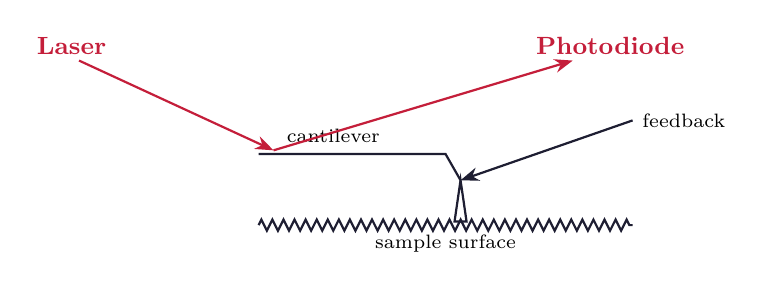
\begin{tikzpicture}[scale=0.95]
  % laser source
  \node[font=\small\bfseries, color=myred] at (0.5,3.4) {Laser};
  \draw[redarrow] (0.6,3.2) -- (3.2,2.0);
  % cantilever
  \draw[thick, mydark] (3.0,1.95) -- (5.5,1.95) -- (5.7,1.6);
  \node[font=\scriptsize] at (4.0,2.2) {cantilever};
  % tip
  \draw[thick, mydark] (5.7,1.6) -- (5.78,1.05) -- (5.62,1.05) -- cycle;
  % sample surface (rough)
  \draw[thick, mydark, decorate, decoration={zigzag, segment length=4pt, amplitude=2pt}]
        (3.0,1.0) -- (8.0,1.0);
  \node[font=\scriptsize] at (5.5,0.75) {sample surface};
  % reflected laser to detector
  \draw[redarrow] (3.2,2.0) -- (7.2,3.2);
  \node[font=\small\bfseries, color=myred] at (7.7,3.4) {Photodiode};
  % feedback
  \node[font=\scriptsize, anchor=west] at (8.0,2.4) {feedback};
  \draw[arrow] (8.0,2.4) -- (5.7,1.6);
\end{tikzpicture}
\end{tcolorbox}

\textbf{Modes of AFM:}
\begin{itemize}[leftmargin=*, itemsep=1pt, topsep=2pt]
  \item \emph{Contact mode}: tip drags on surface; high resolution but can damage soft samples.
  \item \emph{Tapping mode}: cantilever oscillates near resonance, tip touches lightly; safe for biology and polymers.
  \item \emph{Non-contact mode}: tip senses long-range forces; lowest damage.
\end{itemize}

\textbf{Advantages of AFM:} works in air, liquid, and vacuum; no special coating; gives true 3D height; image biological molecules (DNA, proteins) directly.

\subsection{Comparison of Major Surface Techniques}
\begin{tabularx}{\linewidth}{|B{2.4cm}|Y|Y|Y|}
\hline
\textbf{Feature} & \textbf{SEM} & \textbf{AFM} & \textbf{XPS} \\
\hline
Probe & Electrons & Mechanical tip & Soft X-rays \\
\hline
Signal & SE / BSE & Force / deflection & Photo-electrons \\
\hline
Lateral resolution & $\sim 1\ \mathrm{nm}$ & $\sim 0.1\ \mathrm{nm}$ (atomic) & $\sim 10\ \mu\mathrm{m}$ (small spot $\sim 10\ \mu\mathrm{m}$) \\
\hline
Depth probed & Few nm (SE) & Top atomic layer & 5--10 nm \\
\hline
Vacuum & High vacuum & Air / liquid OK & Ultra-high vacuum \\
\hline
Sample preparation & Coat if non-conductive & Almost none & Conductive desirable \\
\hline
Composition info & Possible with EDX & No (height only) & Yes, with chemical state \\
\hline
\end{tabularx}

\subsection{TEM vs SEM}
The two electron-beam microscopies are complementary: SEM gives surface topography while TEM gives internal structure with atomic resolution.

\begin{tabularx}{\linewidth}{|B{2.4cm}|Y|Y|}
\hline
\textbf{Feature} & \textbf{SEM} & \textbf{TEM} \\
\hline
Beam energy & $5$--$30\ \mathrm{kV}$ & $100$--$300\ \mathrm{kV}$ \\
\hline
What is detected & Secondary / back-scattered electrons \emph{above} sample & Electrons \emph{transmitted through} thin sample \\
\hline
Sample form & Bulk, polished, conductive coating if needed & Ultra-thin film ($<100\ \mathrm{nm}$) on grid \\
\hline
Resolution & $\sim 1\ \mathrm{nm}$ & $0.1$--$0.2\ \mathrm{nm}$ (atomic in HRTEM) \\
\hline
Image gives & Topography, depth of field, morphology & Internal structure, lattice fringes, defects \\
\hline
Diffraction option & Limited (EBSD) & Selected-area electron diffraction (SAED) \\
\hline
\end{tabularx}

\subsection{Scanning Tunnelling Microscopy (STM)}
STM achieves true atomic resolution on conducting surfaces by exploiting the quantum tunnelling current that flows between a sharp metal tip and the surface when separated by $\sim 1\ \mathrm{nm}$.

\begin{tcolorbox}[formulabox, title={Tunnelling Current in STM}]
\[
I_{T} \propto V\,\exp(-2\kappa d), \qquad \kappa=\sqrt{\frac{2m_e\phi}{\hbar^{2}}}
\]
$V$ = bias voltage; $d$ = tip--surface gap; $\phi$ = work function. Because $I_T$ falls off exponentially with $d$, a $0.1\ \mathrm{nm}$ change in $d$ changes $I_T$ by a factor of $\sim 10$ — that is the source of atomic-scale sensitivity.
\end{tcolorbox}

\textbf{STM operating modes:}
\begin{itemize}[leftmargin=*, itemsep=1pt, topsep=2pt]
  \item Constant-current mode: feedback adjusts $z$ to keep $I_T$ fixed; image is the $z(x,y)$ map.
  \item Constant-height mode: tip $z$ is fixed; image is the $I_T(x,y)$ map; faster but only safe on flat samples.
\end{itemize}

\textbf{Limitation:} STM only works on conductors and semiconductors, while AFM works on insulators too. STM is the original ``atomic resolution'' technique that won Binnig and Rohrer the 1986 Nobel Prize.

\subsection{BET Surface Area Analysis}
The Brunauer--Emmett--Teller (BET) isotherm extends the Langmuir model to multilayer adsorption and lets you compute the specific surface area of a porous solid from $\mathrm{N_2}$ adsorption at $77\ \mathrm{K}$.

\begin{tcolorbox}[formulabox, title={BET Equation}]
\[
\frac{P/P_0}{V(1-P/P_0)} = \frac{1}{V_m C} + \frac{C-1}{V_m C}\!\left(\frac{P}{P_0}\right)
\]
$P/P_0$ = relative pressure; $V$ = adsorbed volume at $P/P_0$; $V_m$ = monolayer volume; $C$ = BET constant.\\
A plot of LHS vs $P/P_0$ is linear in the range $0.05$--$0.30$. From the slope and intercept, $V_m$ is obtained, and the specific surface area is
\[
S_{\mathrm{BET}} = \frac{V_m\,N_A\,a_m}{V_{\mathrm{molar}}}
\]
where $a_m\approx 0.162\ \mathrm{nm^{2}}$ is the cross-sectional area of an $\mathrm{N_2}$ molecule.
\end{tcolorbox}

\textbf{Why important:} BET surface area is the standard metric for catalysts (Pt/$\gamma$-$\mathrm{Al_2O_3}$ \\$\sim 200\ \mathrm{m^{2}/g}$), zeolites ($\sim 600\ \mathrm{m^{2}/g}$), activated carbon ($>1000\ \mathrm{m^{2}/g}$), and metal-organic frameworks (up to $7000\ \mathrm{m^{2}/g}$).

\subsection{Contact-Angle Measurement: Surface Wettability}
A drop of water on a clean surface forms a contact angle $\theta$ with the surface. This single number is a powerful surface characterisation tool.

\begin{tcolorbox}[formulabox, title={Young's Equation}]
\[
\gamma_{SV}=\gamma_{SL}+\gamma_{LV}\cos\theta
\]
$\gamma_{SV}, \gamma_{SL}, \gamma_{LV}$ = solid--vapour, solid--liquid, liquid--vapour interfacial tensions.\\
\textbf{Hydrophilic} surface: $\theta<90^\circ$ (water spreads). \textbf{Hydrophobic} surface: $\theta>90^\circ$ (water beads). \textbf{Superhydrophobic} (lotus leaf): $\theta>150^\circ$.
\end{tcolorbox}

\textbf{Applications:} surface treatment of biomaterials, anti-fouling coatings, microfluidic device design, paint-adhesion checks.

\begin{tcolorbox}[exambox, title={Exam Points (Section 6)}]
\begin{itemize}[leftmargin=*, itemsep=2pt, topsep=2pt]
  \item Distinguish surface from bulk techniques and explain why probe penetration matters.
  \item For SEM: mention gun, lenses, scan coils, SE/BSE detectors, vacuum.
  \item Quote the XPS equation $E_B=h\nu-E_K-\phi$ and one application (oxidation state).
  \item Sketch AFM tip + cantilever + laser + photodiode.
  \item TEM gives internal structure ($0.1\ \mathrm{nm}$); SEM gives surface topography ($1\ \mathrm{nm}$).
  \item STM tunnelling current $I_T \propto \exp(-2\kappa d)$; works only on conductors.
  \item BET surface area uses $\mathrm{N_2}$ adsorption at $77\ \mathrm{K}$; activated carbon $> 1000\ \mathrm{m^{2}/g}$.
  \item Contact angle: $<90^\circ$ hydrophilic, $>90^\circ$ hydrophobic, $>150^\circ$ superhydrophobic.
\end{itemize}
\end{tcolorbox}

% ===============================================================================
\section{Diffraction and Scattering}
% ===============================================================================

\begin{tcolorbox}[defbox]
\textbf{Diffraction} is the constructive interference of waves scattered by a regular array of atoms or molecules. It produces sharp peaks and is the principal tool for determining crystal structure. \textbf{Scattering} more generally is the redirection of radiation by particles, with or without change of energy; it gives information about size, shape and electron distribution of the scatterers.
\end{tcolorbox}

\subsection{Bragg's Law of X-ray Diffraction}
A crystal acts like a 3D grating because atoms lie on parallel planes separated by an interplanar spacing $d$. Constructive interference occurs at angles satisfying Bragg's law.

\begin{tcolorbox}[formulabox, title={Bragg's Law}]
\[
n\lambda = 2d\sin\theta
\]
$n$ = order (integer); $\lambda$ = wavelength of X-ray (typically Cu~K$\alpha$, $1.5418\,\text{\AA}$); $d$ = interplanar spacing; $\theta$ = Bragg angle (half of the diffraction angle $2\theta$).
\end{tcolorbox}

\begin{tcolorbox}[tikzbox, title={Bragg Reflection from Two Lattice Planes}]
\centering
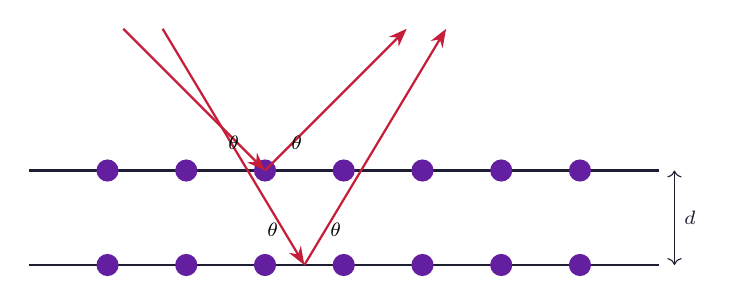
\begin{tikzpicture}[scale=1.0]
  % atomic planes
  \draw[thick, mydark] (0,0) -- (8.0,0);
  \draw[thick, mydark] (0,1.2) -- (8.0,1.2);
  \foreach \x in {1,2,3,4,5,6,7} \fill[mypurple] (\x,0) circle (4pt);
  \foreach \x in {1,2,3,4,5,6,7} \fill[mypurple] (\x,1.2) circle (4pt);
  % d label
  \draw[<->, mydark] (8.2,0) -- (8.2,1.2) node[midway, right, font=\scriptsize] {$d$};
  % incoming/outgoing rays
  \draw[redarrow] (1.2,3.0) -- (3.0,1.2);
  \draw[redarrow] (3.0,1.2) -- (4.8,3.0);
  \draw[redarrow] (1.7,3.0) -- (3.5,0.0);
  \draw[redarrow] (3.5,0.0) -- (5.3,3.0);
  % theta arcs / labels
  \node[font=\scriptsize] at (2.6,1.55) {$\theta$};
  \node[font=\scriptsize] at (3.4,1.55) {$\theta$};
  \node[font=\scriptsize] at (3.1,0.45) {$\theta$};
  \node[font=\scriptsize] at (3.9,0.45) {$\theta$};
\end{tikzpicture}
\end{tcolorbox}

\textbf{Path difference:} The lower ray travels an extra $2d\sin\theta$. Constructive interference (bright spot) requires this to equal $n\lambda$.

\begin{tcolorbox}[examplebox, title={Solved Example: Spacing of NaCl from Bragg Reflection}]
\textbf{Problem:} A first-order ($n=1$) Bragg reflection from NaCl is observed at $\theta=15.5^{\circ}$ with Cu~K$\alpha$ X-rays ($\lambda=0.154\ \mathrm{nm}$). Find the interplanar spacing.

\textbf{Solution:}
\[
d=\frac{n\lambda}{2\sin\theta}=\frac{1\times 0.154}{2\times \sin 15.5^{\circ}}=\frac{0.154}{2\times 0.2672}=0.288\ \mathrm{nm}
\]
This corresponds to the $(200)$ planes of NaCl.
\end{tcolorbox}

\subsection{Powder X-ray Diffraction (PXRD)}
A polycrystalline powder presents all crystallographic orientations to the beam. Each $\{hkl\}$ plane satisfying Bragg's law produces a cone of diffracted intensity, recorded as a series of peaks vs $2\theta$.

\textbf{Information from a powder pattern:}
\begin{itemize}[leftmargin=*, itemsep=1pt, topsep=2pt]
  \item Identification of phases (matched against the ICDD database).
  \item Lattice parameters from peak positions.
  \item Crystallite size from peak broadening (Scherrer formula).
  \item Quantitative phase analysis (Rietveld refinement).
\end{itemize}

\begin{tcolorbox}[formulabox, title={Scherrer Equation for Crystallite Size}]
\[
D=\frac{K\lambda}{\beta\cos\theta}
\]
$D$ = average crystallite size; $K\approx 0.9$ (shape factor); $\beta$ = full-width at half-maximum (FWHM) in radians; $\theta$ = Bragg angle.
\end{tcolorbox}

\subsection{Block Diagram of an X-ray Diffractometer}
\begin{tcolorbox}[tikzbox, title={Block Diagram of a Powder Diffractometer}]
\centering
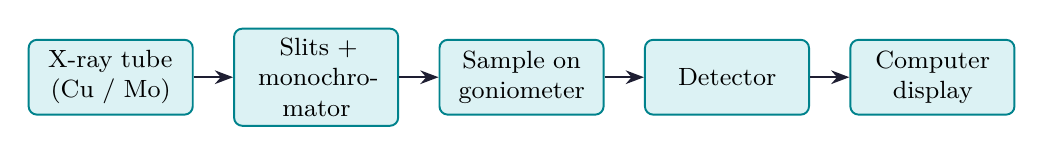
\begin{tikzpicture}[node distance=0.3cm and 0.45cm,
  sblock/.style={rectangle, draw=myteal, fill=hdrteal, text width=1.85cm,
    align=center, minimum height=0.95cm, font=\small,
    rounded corners=3pt, line width=0.7pt}]
  \node[sblock] (n1) {X-ray tube\\(Cu / Mo)};
  \node[sblock, right=0.5cm of n1] (n2) {Slits +\\monochromator};
  \node[sblock, right=0.5cm of n2] (n3) {Sample on goniometer};
  \node[sblock, right=0.5cm of n3] (n4) {Detector};
  \node[sblock, right=0.5cm of n4] (n5) {Computer\\display};
  \draw[arrow] (n1)--(n2);
  \draw[arrow] (n2)--(n3);
  \draw[arrow] (n3)--(n4);
  \draw[arrow] (n4)--(n5);
\end{tikzpicture}
\end{tcolorbox}

\subsection{Electron and Neutron Diffraction}
\begin{tabularx}{\linewidth}{|B{2.4cm}|Y|Y|}
\hline
\textbf{Probe} & \textbf{Wavelength} & \textbf{Speciality} \\
\hline
X-ray & $0.05$--$0.3\ \mathrm{nm}$ & Senses electron density; routine crystallography. \\
\hline
Electron & $\sim 0.005\ \mathrm{nm}$ at 100 kV & Strongly absorbed; ideal for thin films and TEM. \\
\hline
Neutron & $0.1$--$0.3\ \mathrm{nm}$ & Senses nuclear positions, locates light atoms (H, Li); resolves magnetic structure. \\
\hline
\end{tabularx}

\subsection{Rayleigh and Raman Scattering}
When light passes through a transparent medium, a small fraction is scattered. Most of the scattered photons retain the original frequency (\emph{Rayleigh}, elastic). A tiny fraction exchanges energy with molecular vibrations (\emph{Raman}, inelastic).

\begin{tcolorbox}[tikzbox, title={Rayleigh, Stokes and Anti-Stokes Lines in Raman}]
\centering
\begin{tikzpicture}[scale=0.95]
  \draw[->, thick] (0,0) -- (10.4,0) node[right, font=\small] {$\bar{\nu}$};
  \draw[thick, myteal] (5.0,0) -- (5.0,2.4); \node[font=\scriptsize, color=myteal] at (5.0,2.7) {Rayleigh};
  \draw[thick, myred]  (3.4,0) -- (3.4,1.4); \node[font=\scriptsize, color=myred]  at (3.4,1.6) {Stokes};
  \draw[thick, myred]  (6.6,0) -- (6.6,0.7); \node[font=\scriptsize, color=myred]  at (6.6,0.9) {anti-Stokes};
  \draw[<->, dashed, mydark] (5.0,-0.5) -- (3.4,-0.5);
  \node[font=\scriptsize] at (4.2,-0.85) {$+\bar{\nu}_{\text{vib}}$};
  \draw[<->, dashed, mydark] (5.0,-0.5) -- (6.6,-0.5);
  \node[font=\scriptsize] at (5.8,-0.85) {$-\bar{\nu}_{\text{vib}}$};
\end{tikzpicture}
\end{tcolorbox}

\textbf{Raman selection rule:} the vibration must change the molecular polarisability. Combined with the IR rule (dipole change), Raman and IR are often \emph{complementary}.

\begin{tcolorbox}[formulabox, title={Rayleigh Intensity Dependence}]
\[
I_{\mathrm{scat}}\propto \frac{1}{\lambda^{4}}
\]
This $\lambda^{-4}$ dependence explains why the sky is blue (short wavelengths scatter more) and why sunsets are red.
\end{tcolorbox}

\subsection{Other Scattering Techniques}
\begin{tabularx}{\linewidth}{|B{3.0cm}|Y|}
\hline
\textbf{Technique} & \textbf{Information} \\
\hline
Small-angle X-ray scattering (SAXS) & Particle size, shape, $1$--$100\ \mathrm{nm}$ aggregates, polymers. \\
\hline
Dynamic light scattering (DLS) & Hydrodynamic radius and diffusion of nanoparticles in solution. \\
\hline
Static light scattering (SLS) & Molar mass and radius of gyration of polymers (Zimm plot). \\
\hline
Surface-enhanced Raman (SERS) & Trace molecule detection on rough Ag/Au surfaces; single-molecule sensitivity. \\
\hline
\end{tabularx}

\subsection{Applications of Diffraction and Scattering}
\begin{itemize}[leftmargin=*, itemsep=2pt, topsep=2pt]
  \item Crystal-structure determination of metals, ceramics, drugs and proteins.
  \item Phase identification in alloys and minerals.
  \item Quality control of pharmaceuticals (polymorphs).
  \item Thin-film analysis (texture, residual stress) by glancing-incidence XRD.
  \item Particle-size and aggregation studies (DLS, SAXS).
  \item Vibrational fingerprinting using Raman; complements IR.
\end{itemize}

\subsection{Three Classical X-ray Diffraction Methods}
There are three historical setups, each suited to a different sample form.

\begin{tabularx}{\linewidth}{|B{2.6cm}|Y|Y|}
\hline
\textbf{Method} & \textbf{Sample} & \textbf{What is varied} \\
\hline
Laue method & Single crystal, fixed orientation & Polychromatic X-rays (white beam); each plane satisfies Bragg at its own $\lambda$. Used to find crystal symmetry and orient single crystals. \\
\hline
Rotating-crystal method & Single crystal mounted on a goniometer & Crystal rotated; monochromatic $\lambda$. Records reflections from all planes during rotation. \\
\hline
Debye--Scherrer (powder) method & Polycrystalline powder & Random orientations present every plane to the beam; monochromatic $\lambda$. Produces concentric cones, recorded as a $2\theta$ pattern. Most common in materials labs. \\
\hline
\end{tabularx}

\subsection{Raman Effect: Quantum Picture}
Stokes and anti-Stokes lines arise because the molecule can either gain (anti-Stokes) or lose (Stokes) one vibrational quantum during the inelastic scattering event.

\begin{tcolorbox}[formulabox, title={Stokes / Anti-Stokes Intensity Ratio}]
\[
\frac{I_{\text{anti-Stokes}}}{I_{\text{Stokes}}} = \!\left(\frac{\bar{\nu}_0+\bar{\nu}_v}{\bar{\nu}_0-\bar{\nu}_v}\right)^{\!4}\exp\!\left(-\frac{hc\,\bar{\nu}_v}{k_B T}\right)
\]
At room temperature anti-Stokes lines are much weaker because few molecules occupy the $v=1$ state. Heating the sample increases the anti-Stokes/Stokes ratio --- an old way to measure local temperature.
\end{tcolorbox}

\subsection{Why the Sky is Blue: A Worked Rayleigh Calculation}
Sunlight contains all visible wavelengths. Each colour scatters with intensity $\propto 1/\lambda^{4}$.

\begin{tcolorbox}[examplebox, title={Solved Example: Blue / Red Scattering Ratio}]
\textbf{Problem:} Compare the Rayleigh-scattered intensity of blue ($\lambda=470\ \mathrm{nm}$) and red ($\lambda=650\ \mathrm{nm}$) light.

\textbf{Solution:}
\[
\frac{I_{\mathrm{blue}}}{I_{\mathrm{red}}}=\!\left(\frac{650}{470}\right)^{\!4}=(1.383)^{4}=3.66
\]
Blue light is scattered $\sim 3.7\times$ more strongly than red. When you look up away from the sun, you see this scattered blue light; when you look directly at sunset/sunrise the direct beam has been depleted of blue and appears red.
\end{tcolorbox}

\subsection{Raman Spectroscopy: Practical Applications}
Beyond the engineering chemistry textbook, Raman is now a workhorse technique in industry and forensics.

\begin{itemize}[leftmargin=*, itemsep=1pt, topsep=2pt]
  \item Pharmaceutical quality control: through-bottle identification of API and excipients (TRS technology).
  \item Polymorph screening in drug formulation.
  \item Forensic analysis of paints, fibres, narcotics --- non-destructive, no sample prep.
  \item Identification of pigments in art and archaeology (no sampling of priceless objects).
  \item Carbon-material characterisation: D, G and 2D bands in graphene/CNT.
  \item Biomedical Raman: in-vivo cancer margin detection (handheld probes).
  \item SERS for trace explosives and pesticide residue detection.
\end{itemize}

\begin{tcolorbox}[masonbox, title={IR vs Raman: Complementary Spectra of \texorpdfstring{$\mathrm{CO_2}$}{CO2}}]
$\mathrm{CO_2}$ has four vibrational modes. The symmetric stretch is Raman-active (IR-inactive), while the asymmetric stretch and the two bends are IR-active (Raman-inactive). Together IR + Raman map all modes — a direct application of the mutual exclusion principle.
\end{tcolorbox}

\begin{tcolorbox}[exambox, title={Exam Points (Section 7)}]
\begin{itemize}[leftmargin=*, itemsep=2pt, topsep=2pt]
  \item Always state Bragg's law with all symbols defined.
  \item Mention the use of Cu~K$\alpha$ ($\lambda=1.54\,\text{\AA}$) and that we measure peak position $2\theta$.
  \item For nanoparticles, recall Scherrer's equation $D=K\lambda/(\beta\cos\theta)$.
  \item Distinguish Rayleigh (elastic) vs Raman (inelastic) and link to selection rules.
  \item Quote the $1/\lambda^{4}$ Rayleigh law and ``why the sky is blue''.
  \item Three classical XRD methods: Laue (single crystal, polychromatic), rotating-crystal, Debye--Scherrer (powder).
  \item Anti-Stokes/Stokes intensity ratio depends on temperature --- thermometry application.
  \item SERS gives single-molecule sensitivity for forensic and trace detection.
\end{itemize}
\end{tcolorbox}

\newpage
\enlargethispage{2\baselineskip}
\begin{center}
  {\large\bfseries\color{myred} Quick Revision --- Module 2}\\[3pt]
  {\small\color{mydark} Spectroscopic Techniques and Applications $|$ BS-CH101}
\end{center}
\noindent{\color{myred}\rule{\linewidth}{1.2pt}}
\vspace{4pt}

\begin{tcolorbox}[formulabox, title={Key Formulas at a Glance}]
\begin{tabularx}{\linewidth}{|B{4.4cm}|Y|}
\hline
\textbf{Formula / Rule} & \textbf{Meaning} \\
\hline
$E=h\nu=\displaystyle\frac{hc}{\lambda}=hc\bar{\nu}$ & Photon energy in terms of $\nu, \lambda, \bar{\nu}$. \\
\hline
$\Delta E=h\nu$ & Bohr resonance condition for absorption / emission. \\
\hline
$P_{1\to 2}\propto |\mu_{12}|^{2}$ & Transition probability; selection rules emerge here. \\
\hline
$\dfrac{N_2}{N_1}=\dfrac{g_2}{g_1}\,e^{-\Delta E/k_B T}$ & Boltzmann level population. \\
\hline
$A=\varepsilon c l$ & Beer--Lambert law for UV-Vis quantitation. \\
\hline
$\Phi_F=\dfrac{k_F}{k_F+k_{NR}+k_{ISC}}$ & Fluorescence quantum yield. \\
\hline
$\dfrac{F_0}{F}=1+K_{SV}[Q]$ & Stern--Volmer quenching. \\
\hline
$\bar{B}=\dfrac{h}{8\pi^{2}cI}$, $\,I=\mu r^{2}$ & Rotational constant and moment of inertia. \\
\hline
$E_v=(v+\tfrac12)h\nu_0$ & Harmonic-oscillator vibrational energy. \\
\hline
$\bar{\nu}_0=\dfrac{1}{2\pi c}\sqrt{\dfrac{k}{\mu}}$ & Vibrational wavenumber. \\
\hline
$\nu_L=\dfrac{\gamma B_0}{2\pi}$ & NMR Larmor (resonance) frequency. \\
\hline
$\delta\,(\mathrm{ppm})=\dfrac{\nu_{\text{sample}}-\nu_{\text{TMS}}}{\nu_{\text{spec}}}\times 10^{6}$ & NMR chemical shift relative to TMS. \\
\hline
$E_B=h\nu-E_K-\phi$ & XPS binding-energy equation. \\
\hline
$n\lambda=2d\sin\theta$ & Bragg's law for X-ray diffraction. \\
\hline
$D=\dfrac{K\lambda}{\beta\cos\theta}$ & Scherrer equation, crystallite size. \\
\hline
$I_{\text{scat}}\propto 1/\lambda^{4}$ & Rayleigh scattering law. \\
\hline
$\lambda_{\max} = \lambda_{\mathrm{base}} + \sum \text{increments}$ & Woodward--Fieser empirical prediction. \\
\hline
$E = \displaystyle\frac{R_0^{6}}{R_0^{6}+r^{6}}$ & FRET efficiency. \\
\hline
$\displaystyle\frac{\bar{\nu}_{\mathrm{D}}}{\bar{\nu}_{\mathrm{H}}} = \sqrt{\mu_{\mathrm{H}}/\mu_{\mathrm{D}}}$ & Isotope shift ($\approx 1/\sqrt{2}$ for X--H/X--D). \\
\hline
$\Phi_F = k_F\,\tau_F$ & Quantum-yield/lifetime relation. \\
\hline
$\displaystyle\frac{A_{21}}{B_{21}}=\frac{8\pi h\nu^{3}}{c^{3}}$ & Einstein A/B coefficient ratio. \\
\hline
$I_T \propto \exp(-2\kappa d)$ & STM tunnelling current (atomic resolution). \\
\hline
$\gamma_{SV}=\gamma_{SL}+\gamma_{LV}\cos\theta$ & Young's equation for contact angle. \\
\hline
$S_{\mathrm{BET}}=\displaystyle\frac{V_m N_A a_m}{V_{\mathrm{molar}}}$ & BET specific surface area. \\
\hline
\end{tabularx}
\end{tcolorbox}

\begin{tcolorbox}[defbox, title={One-Line Definitions}]
\begin{itemize}[leftmargin=*, itemsep=2pt, topsep=2pt]
  \item \textbf{Spectroscopy:} Study of interaction of EM radiation with matter.
  \item \textbf{Selection rule:} Quantum-number condition that decides whether a transition is allowed.
  \item \textbf{Chromophore:} Functional group responsible for absorption of UV-Vis light.
  \item \textbf{Auxochrome:} Saturated group that shifts and intensifies an existing chromophore.
  \item \textbf{Bathochromic shift:} Movement of $\lambda_{\max}$ to longer wavelength (red shift).
  \item \textbf{Fluorescence:} Spin-allowed radiative emission from $S_1$ to $S_0$.
  \item \textbf{Phosphorescence:} Radiative $T_1\to S_0$ emission, long-lived afterglow.
  \item \textbf{Stokes shift:} Difference between absorption and emission maxima.
  \item \textbf{Quantum yield ($\Phi_F$):} Fraction of absorbed photons re-emitted as fluorescence.
  \item \textbf{Rotational constant ($\bar{B}$):} Inverse moment of inertia in $\mathrm{cm^{-1}}$.
  \item \textbf{Reduced mass ($\mu$):} $m_1 m_2/(m_1+m_2)$ for a diatomic molecule.
  \item \textbf{Force constant ($k$):} Stiffness of a bond modelled as a spring.
  \item \textbf{Chemical shift ($\delta$):} NMR resonance position relative to TMS, in ppm.
  \item \textbf{Larmor frequency:} Resonance $\nu$ of a nuclear spin in a field $B_0$.
  \item \textbf{MRI gradient:} Linear field variation that encodes spatial position.
  \item \textbf{Bragg angle:} Half of the diffraction angle at which constructive interference occurs.
  \item \textbf{Crystallite size (Scherrer):} Average coherent domain size estimated from peak broadening.
  \item \textbf{Rayleigh scattering:} Elastic redirection of light by sub-wavelength particles.
  \item \textbf{Raman scattering:} Inelastic scattering with vibrational energy exchange.
  \item \textbf{Mutual exclusion principle:} For molecules with a centre of symmetry, IR-active modes are Raman-inactive and vice-versa.
  \item \textbf{Franck--Condon principle:} Electronic transitions are vertical because nuclei do not move on the timescale of electronic excitation.
  \item \textbf{Einstein coefficients:} Three rate constants $A_{21}, B_{12}, B_{21}$ describing spontaneous emission, stimulated absorption and stimulated emission.
  \item \textbf{Kasha's rule:} Emission always originates from the lowest excited state of a given multiplicity.
  \item \textbf{FRET:} Distance-dependent non-radiative dipole--dipole energy transfer; $E\propto 1/r^{6}$.
  \item \textbf{Woodward--Fieser rules:} Empirical formula to predict $\lambda_{\max}$ of dienes and enones.
  \item \textbf{Isosbestic point:} Wavelength where two interconverting species have equal $\varepsilon$.
  \item \textbf{Coupling constant ($J$):} Spacing within a multiplet in Hz; independent of $B_0$.
  \item \textbf{Integration:} Area under an NMR signal, proportional to the number of equivalent protons.
  \item \textbf{Ring-current effect:} Aromatic $\pi$-electron circulation deshields ring protons.
  \item \textbf{Gd-DTPA:} Gadolinium chelate used as $T_1$-shortening MRI contrast agent.
  \item \textbf{BET surface area:} Specific surface area measured by $\mathrm{N_2}$ adsorption at $77\ \mathrm{K}$.
  \item \textbf{STM:} Atomic-resolution microscopy based on quantum tunnelling current between tip and conducting surface.
  \item \textbf{Contact angle:} Angle a liquid drop makes with a solid surface; quantifies wettability.
  \item \textbf{Laue method:} Single-crystal XRD with a polychromatic beam, used to determine crystal orientation.
\end{itemize}
\end{tcolorbox}

\begin{tcolorbox}[exambox, title={Frequently Asked / Viva Questions}]
\begin{enumerate}[topsep=0pt, label=\textbf{Q\arabic*.}, itemsep=5pt]
  \item \Q{State the principle of spectroscopy.}
    A molecule absorbs a photon when its energy matches the gap between two allowed levels: $\Delta E = h\nu$.
  \item \Q{What are gross and specific selection rules?}
    Gross rule sets a property the molecule must have (dipole, polarisability, spin), specific rule restricts the change in quantum numbers (e.g.\ $\Delta v=\pm 1$).
  \item \Q{Why is $\mathrm{N_2}$ IR-inactive but Raman-active?}
    The $\mathrm{N_2}$ stretch does not change the dipole moment (zero) but does change polarisability.
  \item \Q{State Beer--Lambert law and one limitation.}
    $A=\varepsilon c l$. It fails at high concentration because intermolecular interactions alter $\varepsilon$.
  \item \Q{Define chromophore and give two examples.}
    Unsaturated group responsible for UV-Vis absorption; e.g.\ $\mathrm{C{=}O}$, $\mathrm{C{=}C}$.
  \item \Q{What is the difference between fluorescence and phosphorescence?}
    Fluorescence is spin-allowed $S_1\to S_0$ ($10^{-9}$--$10^{-7}\ \mathrm{s}$); phosphorescence is spin-forbidden $T_1\to S_0$ ($10^{-3}$--$10\ \mathrm{s}$).
  \item \Q{Name two medical uses of fluorescence.}
    Fluorescein retinal angiography and photodynamic therapy of cancer.
  \item \Q{Why does $\mathrm{HCl}$ show a microwave spectrum but $\mathrm{H_2}$ does not?}
    Only $\mathrm{HCl}$ has a permanent electric dipole; the rotational gross rule fails for $\mathrm{H_2}$.
  \item \Q{State the harmonic-oscillator selection rule for IR.}
    $\Delta v = \pm 1$, with the requirement that the vibration changes the dipole moment.
  \item \Q{State the Larmor equation.}
    $\nu_L=\gamma B_0/(2\pi)$; for $^{1}\mathrm{H}$ at $11.74\ \mathrm{T}$, $\nu_L=500\ \mathrm{MHz}$.
  \item \Q{What is chemical shift in NMR?}
    Position of a resonance in ppm relative to TMS: $\delta=(\nu_s-\nu_{\mathrm{TMS}})/\nu_{\mathrm{spec}}\times 10^{6}$.
  \item \Q{How does MRI distinguish tissues?}
    Through differences in proton density, $T_1$ and $T_2$ relaxation times of water in each tissue.
  \item \Q{Give two surface techniques and one piece of information each.}
    SEM (topography), XPS (oxidation state of surface atoms).
  \item \Q{State Bragg's law.}
    $n\lambda = 2d\sin\theta$; gives $d$-spacings of crystal planes from peak positions.
  \item \Q{Differentiate Rayleigh and Raman scattering.}
    Rayleigh is elastic, same $\nu$. Raman is inelastic, $\pm \bar{\nu}_{\mathrm{vib}}$ shifted lines.
  \item \Q{State Franck--Condon principle.}
    Electronic transitions are vertical on a potential-energy diagram because nuclei do not move during the $10^{-15}\ \mathrm{s}$ duration of electronic absorption.
  \item \Q{What does Kasha's rule state?}
    Emission almost always originates from the lowest vibrational level of the lowest excited state of a given spin multiplicity, regardless of the excitation wavelength.
  \item \Q{Define FRET and give one application.}
    Non-radiative resonance energy transfer from an excited donor to a nearby acceptor; $E\propto R_0^{6}/(R_0^{6}+r^{6})$. Used as a molecular ruler in single-molecule biophysics and TaqMan PCR.
  \item \Q{State Woodward--Fieser rules.}
    Empirical addition of base value plus increments for substituents predicts $\lambda_{\max}$ of dienes ($215\ \mathrm{nm}$ acyclic) and $\alpha,\beta$-unsaturated ketones ($215\ \mathrm{nm}$ acyclic) within $\pm 5\ \mathrm{nm}$.
  \item \Q{What is an isosbestic point?}
    Wavelength where two interconverting species have equal $\varepsilon$; presence of a sharp isosbestic point confirms a clean two-component equilibrium.
  \item \Q{Why does $\mathrm{D{-}Cl}$ absorb at lower wavenumber than $\mathrm{H{-}Cl}$?}
    Same force constant but doubled reduced mass; $\bar{\nu}\propto 1/\sqrt{\mu}$ gives a factor of $\sim 0.71$. So DCl absorbs at $\sim 2137\ \mathrm{cm^{-1}}$ vs HCl at $2989\ \mathrm{cm^{-1}}$.
  \item \Q{What information does NMR integration give?}
    Area under a peak is proportional to the number of equivalent protons in that environment, providing the H-count of each chemical type.
  \item \Q{What is the coupling constant $J$ and how do you measure it?}
    Spacing within a multiplet, expressed in Hz, independent of $B_0$. It is read directly from line spacing in the spectrum and is diagnostic of cis/trans, geminal/vicinal coupling.
  \item \Q{Name two MRI contrast agents.}
    Gd-DTPA (Magnevist) shortens water $T_1$ to brighten tissues; SPIONs shorten $T_2$ to darken regions where they accumulate.
  \item \Q{How does STM achieve atomic resolution?}
    Tunnelling current $I_T\propto \exp(-2\kappa d)$ falls off exponentially with tip--surface gap, so a $0.1\ \mathrm{nm}$ change alters the current by $\sim 10\times$.
  \item \Q{What is BET surface area?}
    Specific surface area of porous solids measured from $\mathrm{N_2}$ adsorption at $77\ \mathrm{K}$ using the BET multilayer-isotherm equation. Activated carbon $>1000\ \mathrm{m^{2}/g}$.
  \item \Q{What is the contact angle and what does it tell you?}
    Angle a sessile drop makes with a surface; $<90^\circ$ hydrophilic, $>90^\circ$ hydrophobic, $>150^\circ$ superhydrophobic. Quantifies surface wettability via Young's equation.
  \item \Q{Why is the sky blue and the sunset red?}
    Rayleigh-scattered intensity $\propto 1/\lambda^{4}$, so blue scatters $\sim 3.7\times$ more than red. Looking up reveals scattered blue; the direct sunset beam has been depleted of blue and looks red.
\end{enumerate}
\end{tcolorbox}

\begin{tcolorbox}[tikzbox, title={Summary Reference Table of Spectroscopic Techniques}]
\begin{tabularx}{\linewidth}{|B{3.0cm}|Y|Y|Y|}
\hline
\textbf{Technique} & \textbf{Region / probe} & \textbf{Information} & \textbf{Key formula / rule} \\
\hline
UV-Vis & 200--800 nm photons & Electronic transitions, concentration & $A=\varepsilon c l$ \\
\hline
Fluorescence & UV-Vis emission & Excited state, medical imaging & $\Phi_F$, Stern--Volmer \\
\hline
IR / FT-IR & $400$--$4000\ \mathrm{cm^{-1}}$ & Functional groups & $\bar{\nu}_0=\frac{1}{2\pi c}\sqrt{k/\mu}$ \\
\hline
Microwave & $1$--$300\ \mathrm{GHz}$ & Bond length, $I$, $\bar{B}$ & $\bar{B}=h/(8\pi^{2}cI)$ \\
\hline
NMR & RF in strong $B_0$ & H/C environments, structure & $\nu_L=\gamma B_0/(2\pi)$ \\
\hline
MRI & RF + magnetic gradients & Soft-tissue images & $T_1, T_2$ contrast \\
\hline
SEM / AFM / XPS & Electrons / tip / X-rays & Surface morphology + chemistry & $E_B=h\nu-E_K-\phi$ (XPS) \\
\hline
XRD & X-rays on crystal & Crystal structure, $d$-spacings & $n\lambda=2d\sin\theta$ \\
\hline
Raman & Vis/NIR scattering & Vibrational + symmetry info & Polarisability change \\
\hline
\end{tabularx}
\end{tcolorbox}

\end{document}
